%==============================================================================
% tento soubor pouzijte jako zaklad
% this file should be used as a base for the thesis
% Autoři / Authors: 2008 Michal Bidlo, 2019 Jaroslav Dytrych
% Kontakt pro dotazy a připomínky: sablona@fit.vutbr.cz
% Contact for questions and comments: sablona@fit.vutbr.cz
%==============================================================================
% kodovani: UTF-8 (zmena prikazem iconv, recode nebo cstocs)
% encoding: UTF-8 (you can change it by command iconv, recode or cstocs)
%------------------------------------------------------------------------------
% zpracování / processing: make, make pdf, make clean
%==============================================================================
% Soubory, které je nutné upravit nebo smazat: / Files which have to be edited or deleted:
%   projekt-20-literatura-bibliography.bib - literatura / bibliography
%   projekt-01-kapitoly-chapters.tex - obsah práce / the thesis content
%   projekt-01-kapitoly-chapters-en.tex - obsah práce v angličtině / the thesis content in English
%   projekt-30-prilohy-appendices.tex - přílohy / appendices
%   projekt-30-prilohy-appendices-en.tex - přílohy v angličtině / appendices in English
%==============================================================================
\documentclass[zadani]{fitthesis} % bez zadání - pro začátek práce, aby nebyl problém s překladem
%\documentclass[english]{fitthesis} % without assignment - for the work start to avoid compilation problem
%\documentclass[zadani]{fitthesis} % odevzdani do wisu a/nebo tisk s barevnými odkazy - odkazy jsou barevné
%\documentclass[english,zadani]{fitthesis} % for submission to the IS FIT and/or print with color links - links are color
%\documentclass[zadani,print]{fitthesis} % pro černobílý tisk - odkazy jsou černé
%\documentclass[english,zadani,print]{fitthesis} % for the black and white print - links are black
%\documentclass[zadani,cprint]{fitthesis} % pro barevný tisk - odkazy jsou černé, znak VUT barevný
%\documentclass[english,zadani,cprint]{fitthesis} % for the print - links are black, logo is color
% * Je-li práce psaná v anglickém jazyce, je zapotřebí u třídy použít 
%   parametr english následovně:
%   If thesis is written in English, it is necessary to use 
%   parameter english as follows:
%      \documentclass[english]{fitthesis}
% * Je-li práce psaná ve slovenském jazyce, je zapotřebí u třídy použít 
%   parametr slovak následovně:
%   If the work is written in the Slovak language, it is necessary 
%   to use parameter slovak as follows:
%      \documentclass[slovak]{fitthesis}
% * Je-li práce psaná v anglickém jazyce se slovenským abstraktem apod., 
%   je zapotřebí u třídy použít parametry english a enslovak následovně:
%   If the work is written in English with the Slovak abstract, etc., 
%   it is necessary to use parameters english and enslovak as follows:
%      \documentclass[english,enslovak]{fitthesis}

% Základní balíčky jsou dole v souboru šablony fitthesis.cls
% Basic packages are at the bottom of template file fitthesis.cls
% zde můžeme vložit vlastní balíčky / you can place own packages here

% Kompilace po částech (rychlejší, ale v náhledu nemusí být vše aktuální)
% Compilation piecewise (faster, but not all parts in preview will be up-to-date)
% \usepackage{subfiles}

% Nastavení cesty k obrázkům
% Setting of a path to the pictures
%\graphicspath{{obrazky-figures/}{./obrazky-figures/}}
%\graphicspath{{obrazky-figures/}{../obrazky-figures/}}

%---rm---------------
\renewcommand{\rmdefault}{lmr}%zavede Latin Modern Roman jako rm / set Latin Modern Roman as rm
%---sf---------------
\renewcommand{\sfdefault}{qhv}%zavede TeX Gyre Heros jako sf
%---tt------------
\renewcommand{\ttdefault}{lmtt}% zavede Latin Modern tt jako tt

% vypne funkci šablony, která automaticky nahrazuje uvozovky,
% aby nebyly prováděny nevhodné náhrady v popisech API apod.
% disables function of the template which replaces quotation marks
% to avoid unnecessary replacements in the API descriptions etc.
\csdoublequotesoff



\usepackage{url}
\usepackage{placeins}

% =======================================================================
% balíček "hyperref" vytváří klikací odkazy v pdf, pokud tedy použijeme pdflatex
% problém je, že balíček hyperref musí být uveden jako poslední, takže nemůže
% být v šabloně
% "hyperref" package create clickable links in pdf if you are using pdflatex.
% Problem is that this package have to be introduced as the last one so it 
% can not be placed in the template file.
\ifWis
\ifx\pdfoutput\undefined % nejedeme pod pdflatexem / we are not using pdflatex
\else
  \usepackage{color}
  \usepackage[unicode,colorlinks,hyperindex,plainpages=false,pdftex]{hyperref}
  \definecolor{hrcolor-ref}{RGB}{223,52,30}
  \definecolor{hrcolor-cite}{HTML}{2F8F00}
  \definecolor{hrcolor-urls}{HTML}{092EAB}
  \hypersetup{
	linkcolor=hrcolor-ref,
	citecolor=hrcolor-cite,
	filecolor=magenta,
	urlcolor=hrcolor-urls
  }
  \def\pdfBorderAttrs{/Border [0 0 0] }  % bez okrajů kolem odkazů / without margins around links
  \pdfcompresslevel=9
\fi
\else % pro tisk budou odkazy, na které se dá klikat, černé / for the print clickable links will be black
\ifx\pdfoutput\undefined % nejedeme pod pdflatexem / we are not using pdflatex
\else
  \usepackage{color}
  \usepackage[unicode,colorlinks,hyperindex,plainpages=false,pdftex,urlcolor=black,linkcolor=black,citecolor=black]{hyperref}
  \definecolor{links}{rgb}{0,0,0}
  \definecolor{anchors}{rgb}{0,0,0}
  \def\AnchorColor{anchors}
  \def\LinkColor{links}
  \def\pdfBorderAttrs{/Border [0 0 0] } % bez okrajů kolem odkazů / without margins around links
  \pdfcompresslevel=9
\fi
\fi
% Řešení problému, kdy klikací odkazy na obrázky vedou za obrázek
% This solves the problems with links which leads after the picture
\usepackage[all]{hypcap}

% Informace o práci/projektu / Information about the thesis
%---------------------------------------------------------------------------
\projectinfo{
  %Prace / Thesis
  project={BP},            %typ práce BP/SP/DP/DR  / thesis type (SP = term project)
  year={2021},             % rok odevzdání / year of submission
  date=\today,             % datum odevzdání / submission date
  %Nazev prace / thesis title
  title.cs={Porovnání nástrojů pro vývoj webových aplikací na bázi JavaScriptu},  % název práce v češtině či slovenštině (dle zadání) / thesis title in czech language (according to assignment)
  title.en={Comparison of JavaScript-Based Web Application Development Tools}, % název práce v angličtině / thesis title in english
  %title.length={14.5cm}, % nastavení délky bloku s titulkem pro úpravu zalomení řádku (lze definovat zde nebo níže) / setting the length of a block with a thesis title for adjusting a line break (can be defined here or below)
  %sectitle.length={14.5cm}, % nastavení délky bloku s druhým titulkem pro úpravu zalomení řádku (lze definovat zde nebo níže) / setting the length of a block with a second thesis title for adjusting a line break (can be defined here or below)
  %Autor / Author
  author.name={Jakub},   % jméno autora / author name
  author.surname={Gajdošík},   % příjmení autora / author surname 
  %author.title.p={Bc.}, % titul před jménem (nepovinné) / title before the name (optional)
  %author.title.a={Ph.D.}, % titul za jménem (nepovinné) / title after the name (optional)
  %Ustav / Department
  department={UITS}, % doplňte příslušnou zkratku dle ústavu na zadání: UPSY/UIFS/UITS/UPGM / fill in appropriate abbreviation of the department according to assignment: UPSY/UIFS/UITS/UPGM
  % Školitel / supervisor
  supervisor.name={Janoušek},   % jméno školitele / supervisor name 
  supervisor.surname={Vladimír},   % příjmení školitele / supervisor surname
  supervisor.title.p={doc. Ing.},   %titul před jménem (nepovinné) / title before the name (optional)
  supervisor.title.a={Ph.D.},    %titul za jménem (nepovinné) / title after the name (optional)
  % Klíčová slova / keywords
  keywords.cs={JavaScript, TypeScript, webová aplikace, Angular, Vue}, % klíčová slova v českém či slovenském jazyce / keywords in czech or slovak language
  keywords.en={JavaScript, TypeScript, web application, Angular, Vue}, % klíčová slova v anglickém jazyce / keywords in english
  %keywords.en={Here, individual keywords separated by commas will be written in English.},
  % Abstrakt / Abstract
  abstract.cs={Cílem této práce je prozkoumat moderní proces vývoje webových aplikací. Srovnání postupů a použitých nástrojů při vývoji webové aplikace. Práce bude především zaměřena na nový trend, vývoje webových aplikací pomocí JavaScriptu s použitím různých aplikačních rámců. Práce bude srovnávat dva aplikačních rámce pro vývoj aplikací. }, % abstrakt v českém či slovenském jazyce / abstract in czech or slovak language
  abstract.en={The aim of this work is to explore the modern web application development process. Comparison of procedures and tools used in web application development. The work will be mainly focused on a new trend, web application development using JavaScript using various frameworks. The work will compare two frameworks for application development.}, % abstrakt v anglickém jazyce / abstract in english
  %abstract.en={An abstract of the work in English will be written in this paragraph.},
  % Prohlášení (u anglicky psané práce anglicky, u slovensky psané práce slovensky) / Declaration (for thesis in english should be in english)
  declaration={Prohlašuji, že jsem tuto bakalářskou práci vypracoval samostatně pod vedením pana Doc. Ing. VLADIMÍRJANOUŠEK Ph.D. Uvedl jsem všechny literární prameny, publikace a další zdroje, ze kterých jsem čerpal.},
  %declaration={I hereby declare that this Bachelor's thesis was prepared as an original work by the author under the supervision of Mr. X
% The supplementary information was provided by Mr. Y
% I have listed all the literary sources, publications and other sources, which were used during the preparation of this thesis.},
  % Poděkování (nepovinné, nejlépe v jazyce práce) / Acknowledgement (optional, ideally in the language of the thesis)
  acknowledgment={Chci poděkovat svému vedoucímu, své rodině a přítelkyni.},
  %acknowledgment={Here it is possible to express thanks to the supervisor and to the people which provided professional help
%(external submitter, consultant, etc.).},
  % Rozšířený abstrakt (cca 3 normostrany) - lze definovat zde nebo níže / Extended abstract (approximately 3 standard pages) - can be defined here or below
  %extendedabstract={Do tohoto odstavce bude zapsán rozšířený výtah (abstrakt) práce v českém (slovenském) jazyce.},
  %faculty={FIT}, % FIT/FEKT/FSI/FA/FCH/FP/FAST/FAVU/USI/DEF
  faculty.cs={Fakulta informačních technologií}, % Fakulta v češtině - pro využití této položky výše zvolte fakultu DEF / Faculty in Czech - for use of this entry select DEF above
  faculty.en={Faculty of Information Technology}, % Fakulta v angličtině - pro využití této položky výše zvolte fakultu DEF / Faculty in English - for use of this entry select DEF above
  department.cs={Ústav matematiky}, % Ústav v češtině - pro využití této položky výše zvolte ústav DEF nebo jej zakomentujte / Department in Czech - for use of this entry select DEF above or comment it out
  department.en={Institute of Mathematics} % Ústav v angličtině - pro využití této položky výše zvolte ústav DEF nebo jej zakomentujte / Department in English - for use of this entry select DEF above or comment it out
}

% Rozšířený abstrakt (cca 3 normostrany) - lze definovat zde nebo výše / Extended abstract (approximately 3 standard pages) - can be defined here or above
%\extendedabstract{Do tohoto odstavce bude zapsán výtah (abstrakt) práce v českém (slovenském) jazyce.}

% nastavení délky bloku s titulkem pro úpravu zalomení řádku - lze definovat zde nebo výše / setting the length of a block with a thesis title for adjusting a line break - can be defined here or above
%\titlelength{14.5cm}
% nastavení délky bloku s druhým titulkem pro úpravu zalomení řádku - lze definovat zde nebo výše / setting the length of a block with a second thesis title for adjusting a line break - can be defined here or above
%\sectitlelength{14.5cm}

% řeší první/poslední řádek odstavce na předchozí/následující stránce
% solves first/last row of the paragraph on the previous/next page
\clubpenalty=10000
\widowpenalty=10000

% checklist
\newlist{checklist}{itemize}{1}
\setlist[checklist]{label=$\square$}

\begin{document}
  % Vysazeni titulnich stran / Typesetting of the title pages
  % ----------------------------------------------
  \maketitle
  % Obsah
  % ----------------------------------------------
  \setlength{\parskip}{0pt}

  {\hypersetup{hidelinks}\tableofcontents}
  
  % Seznam obrazku a tabulek (pokud prace obsahuje velke mnozstvi obrazku, tak se to hodi)
  % List of figures and list of tables (if the thesis contains a lot of pictures, it is good)
  \ifczech
    \renewcommand\listfigurename{Seznam obrázků}
  \fi
  \ifslovak
    \renewcommand\listfigurename{Zoznam obrázkov}
  \fi
  % {\hypersetup{hidelinks}\listoffigures}
  
  \ifczech
    \renewcommand\listtablename{Seznam tabulek}
  \fi
  \ifslovak
    \renewcommand\listtablename{Zoznam tabuliek}
  \fi
  % {\hypersetup{hidelinks}\listoftables}

  \ifODSAZ
    \setlength{\parskip}{0.5\bigskipamount}
  \else
    \setlength{\parskip}{0pt}
  \fi

  % vynechani stranky v oboustrannem rezimu
  % Skip the page in the two-sided mode
  \iftwoside
    \cleardoublepage
  \fi

  % Text prace / Thesis text
  % ----------------------------------------------
  
\chapter{Úvod}
Webové aplikace prošly v posledním desetiletí dynamickým vývojem a dnes se stávají podstatnou součástí webu a v širším pojetí také společnosti. Stávají se čím dál častějším typem aplikací a nahrazují nativní desktopové aplikace. Současně mají také svůj podíl na zvyšující se kvalitě a funkcionalitě mnohých webových stránek. Je jednodušší naprogramovat stránky tak, aby byly dynamické, aby se přizpůsobovaly uživateli, nezatěžovaly jeho hardware a aby zlepšovaly jeho uživatelskou zkušenost s interakcí s webovou stránkou či aplikací. Toto umožňuje mimo jiné rychlý vývoj technologií pro tvorbu webových aplikací, což je jedno z nejrychleji se rozvíjejících odvětví v rámci programování. Tyto technologie zároveň nekladou na programátora vysoké nároky a umožňují mu se zaměřit se na více specifické funkce aplikací. Toto je do velké míry zásluha jazyka JavaScript, jeho knihoven a technologií na něm založených.

Nejvýznamnější technologií v této oblasti jsou javascriptové aplikační rámce. Jedná se o softwarovou strukturu, která usnadňuje vývoj aplikace, a to prostřednictvím nástrojů a metodiky obsažené v těchto rámcích. Umožňují vývoj aplikací tak, že je vnitřní logika implementovaná pomocí JavaScriptu a běží tak na straně klienta. Mezi nejpopulárnější rámce patří dnes Angular, Vue a React. Každý z těchto aplikačních rámců nicméně funguje jiným způsobem a hodí se tak k odlišným účelům.

Právě na aplikační rámce Angular a Vue a na rozdíly mezi nimi jsem zaměřil svou práci. Aplikační rámce se dynamicky vyvíjí, v nedávné době například Angular zásadně změnil způsob kompilace kódu skrze nástroj pro kompilace s názvem Ivy. V této práci tak představuji současnou podobu a fungování rámců Angular a Vue. Zároveň se zde soustředím na aktuální srovnání obou rámců prostřednictvím vlastní webové aplikace. Mnohá srovnání se zaměřují na charakteristiky aplikačních rámců v rámci jednoduchých shodných testovacích aplikacích. V této práci chci nicméně představit a porovnat práci s Angularem a Vue používanými v rámci jedné komplexní aplikace. Toto umožní porovnat oba rámce novým způsobem a nahlédnout do jejich fungování. Hlavní část výsledné aplikace tak byla vytvořena za pomocí rámce Angular, do něhož byla vložena webová komponenta vytvořená pomocí Vue.

V práci se nejdříve zaměřuji na webové aplikace - představuji jejich historii, vlastnosti, typy webových aplikací a základní technologie využívané při jejich tvorbě. Dále se věnuji samotnému jazyku JavaScript, u nějž uvádím základní informace a píši o jeho vlastnostech a technologiích, které jsou s ním spjaté. V další části se zabývám samotnými javascriptovými aplikačními rámci a představuji současné fungování nejvýznamnějších rámců, tedy Angularu, Vue a Reactu. Následující kapitola představuje výzkumný záměr a návrh aplikace. Poté popisuji implementaci samotné webové aplikace a její části. Další kapitola je zaměřena na srovnání obou aplikačních rámců na základě zvolených kritérií, po němž svou práci zakončuji závěrem.  
  \chapter{Webové aplikace}
Základní definice webové aplikace je taková, že se jedná o program, k němuž se lze připojit pomocí HTTP (Hyper Text Transfer Protocol), a to pomocí počítačové sítě (Internet) ale i v rámci lokální podoby (Intranet). Vymezení toho, co je a co není webová aplikace, je v dnešní době velmi složité, jelikož existuje velké množství definic, které nemusí souhlasit v každém bodě. Webová aplikace může být totiž více či méně rozvinutá, což komplikuje vytvoření jednotné pojetí. Všechny definice se ale shodují v tom, že webová aplikace je rozšíření webové stránky a že se snaží uživateli zlepšit jeho uživatelskou zkušenost a práci s webovou stránkou. Činí tak za pomoci vnitřní logiky, a sice v rozsahu od jednoduchých filtrů nebo ukládání dat o uživateli, která jsou později zpracovávána, až pro vytváření informačních systémů a online obchodů. Dá se tedy říci, že jde především o zefektivnění a zpřístupnění dat uživateli na základě vstupních informací. Rozdíly mezi webovými aplikacemi a pouhými stránkami mohou být především pro uživatele méně rozpoznatelné, jelikož i jednoduché informativní stránky se dnes běžně snaží o efektivnější a příjemnější komunikaci s uživatelem \cite{differencewebapps}.

Jelikož jsou webové aplikace tak rozsáhlým tématem, je vhodné si kromě definice také ujasnit základní pojmy, s nimiž se často spojují, a vymezit si rozdíly a spojitosti mezi nimi. Webová stránka (website) je kolekce webových stránek a souborů, které jsou uloženy na webovém serveru a jsou dostupné pomocí internetu. Tyto kolekce se nachází pod jednou společnou internetovou doménou pojmenovávající tuto kolekci \cite{website}.

Webový server je pak počítač, který se zaměřuje na odpovídání na HTTP požadavky od klienta a jejich zpracovávání do dokumentu, který je reprezentován webovým stránkami. Tyto úpravy provádí s pomocí aplikačního serveru za účelem vytvoření dynamických stránek. Samotný aplikační server je software, jehož účelem je zpracování stránky za pomocí serverových jazyků, a to před tím než bude zaslána klientovi \cite{webserver}. Aplikační server tak zajišťuje dynamický charakter stránky, přístup k databázi a také vnitřní logiku. Nejpoužívanějším jazykem pro tento způsob zpracování je PHP (Hypertext Preprocessor).

Existuje několik druhů stránek, přičemž nejzákladnější rozdělení v kontextu této práce je členění na statické a dynamické webové stránky. Statické stránky mají jasně daný obsah, který server nikdy nemění, a pouze jej při zažádání zašle uživateli. Je ovšem nutné podotknout, že statické stránky se v dnešní době chovají, jako by byly dynamické, a to díky implementaci skriptů, které umožňují pohyblivost stránky, což v jistém ohledu připomíná dynamické stránky \cite{futureofsoftware}. 
Dynamické stránky jsou oproti tomu proměnlivé. Při zažádání o webovou stránku mohou být zaslány v požadavku dodatečné informace, které přimějí webový server, aby poslal upravenou verzi dané stránky. Aplikační server provede úpravy na stránce a zašle uživateli novou podobu stránky. Tyto úpravy často souvisí se zobrazováním dat z databáze, k níž přistupuje webový server. Získává z ní podstatná data, která poté zpracuje a přeposílá zpátky uživateli. Tato data jsou ukládána především ve formě tabulek \cite{futureofsoftware}.

Samotná webová stránka je reprezentována v podobě dokumentů, k nimž se dá přistoupit skrze internetovou síť (tj. zpravidla prostřednictvím WWW). Jako základ se používá značkovací jazyk HTML a stylování pomocí CSS. Stránka se běžně skládá z informačních textů, videí, obrázků, odkazů a dalších prvků.

    \section{Historie tvorby webových aplikací}
Webové aplikace vzešly z přenosu dat pomocí HTTP (Hypertext Transfer Protocol) mezi klientem a serverem. Tento přenos dat uskutečnil Tim Berners-Lee v roce 1989. O rok později byla vytvořena první webová stránka, která popisovala projekt jako takový a obsahovala návod jak takový přenos dat vytvořit. Tím začala éra World Wide Webu (WWW), tedy celosvětové sítě umožňující okamžitou online komunikaci. Jako první se rozšířila tvorba webových stránek, které obsahovaly pouze text a jejichž účelem bylo předávání odborných informací. Mezi prvními informacemi předávanými tímto způsobem byly výsledky vědeckých výzkumů anebo vládní či vojenské dokumentace. Jediným nástrojem, který v té době tvořil tyto stránky, byl značkovací jazyk HTML (Hypertext Markup Language), který se stal základním kamenem pro veškerou tvorbu na webu \cite{futureofsoftware}. Díky inovativnímu prohlížeči Mosaic bylo možné kromě textu a základních tabulek zobrazovat také obrázky, což umožnilo získat zájem většího okolí a naznačilo cestu pro designový vývoj webu. Z odlišných fontů a barevných schémat začal vznikat nový vzhled webu, u kterého začala nabývat na významu také estetická rovina \cite{webbrowsers}. V první půlce 90. let začalo docházet k vyššímu využití potenciálu, který World Wide Web nabízel, a kromě informačních webů došlo i ke vzniku a rozšíření webových stránek vytvořených ke komerčním účelům. Počet uživatelů rapidně vzrostl na desítky milionů. Díky rostoucímu množství uživatelů bylo čím dál dostupnější internetové připojení a žádná společnost nechtěla být pozadu s dobou. V následujících letech umožnily nové technologie rozvoj tohoto odvětví. Došlo ke vzniku nových významných programovacích jazyků, které se staly základem moderního vývoje webových stránek. Mezi tyto jazyky patří CSS, PHP, JavaScript, Flash a mnohé další.

Během roku 2000 se začala hroutit internetová ekonomika, což bylo zapříčiněno prasknutím ekonomické bubliny a následným poklesem hodnoty akcií řady společností, které se zabývaly technologiemi spojenými s internetem \cite{bubble}. Jakmile došlo ke zotavení trhu po této krizi, začalo docházet k vytváření základů, které později umožnily globální rozšíření webu i pro širokou veřejnost. Počítače začaly být čím dál výkonnější, bylo umožněno vytvářet komplexnější webové stránky a využívat multimédia. Tento technologický rozvoj umožnil vyšší efektivitu stránek, častější využívání vizuálních prvků jako jsou animace anebo videa. Jazyky se tomuto tempu vývoje průběžně přizpůsobovaly a jejich vývojáři se snažili, aby programovací jazyky byly efektivněji využitelné. V této době vznikl především jQuery a AJAX, které nachází své využití i v dnešní době. Vznikly také nejpopulárnější stránky hostující webové aplikace, kterými je mimo jiné Youtube, Twitter anebo Facebook. Roku 2007 byla představena možnost používání internetu na mobilních zařízení díky představení prvního zařízení iPhone vyvinutého společností Apple. Tento bod značí začátek nutnosti řešení dynamického rozlišení a vzhledu stránek, vícedotykového ovládání a vytváření mobilní webové aplikace \cite{futureofsoftware}.

Počítače v té době měly výkon, který postačoval k nutným úkonům, ale zaostávaly zprostředkovací webové prohlížeče.Tvorba webových aplikací je s webovými prohlížeči silně spojena proto, že bez prohlížeče není prakticky možné se k aplikacím připojovat. Vývoj nových prohlížečů nicméně nebyl jednoduchý. Tvůrci prohlížečů se snažili nabídnout svá originální řešení a funkce, což znemožňovalo vznik norem, které by zajistily kompatibilitu napříč prohlížeči. Toto komplikovalo vývoj webových stránek a aplikací v té době, a to především proto, že každý z dostupných prohlížečů zobrazoval webovou stránku odlišně. Některé prohlížeče byly například založeny na různých interpretacích standardů a jiné si vytvářely vlastní značení pro HTML jazyk, který ale nebyl kompatibilní s konkurenčními prohlížeči. Každý také zobrazoval i styloval pomocí CSS jiným způsobem, některé příkazy byly chybně implementované, což vedlo ke značným komplikacím v rámci web designu.

Mezi nejpopulárnější prohlížeče v dnešní době patří s velkým předstihem Chrome od společnosti Google \cite{chrome}. Dalšími široce rozšířenými prohlížeči je Safari vytvořený společností Apple, dále Internet Explorer a Edge spadající pod Microsoft anebo Firefox a Opera vytvořené stejnojmennými společnostmi. Internet Explorer je nejstarším ze stávajících běžných prohlížečů. V druhé polovině 90. let soupeřil s prohlížečem Netscape Navigator, Internet Explorer jej ale předčil technickými vymoženostmi, například první implementací CSS neboli kaskádových stylů. Roku 2002 se objevil nový konkurenční prohlížeč Firefox. Ten byl sice hodnocen kladně, ale Internet Explorer byl tehdy rozšířenější díky popularitě operačního systému Windows, který spadá pod stejnou společnost. V roce 2008 ovšem Google představil svůj prohlížeč Google Chrome, který překonal v následujících čtyřech letech veškeré konkurenční prohlížeče. Chrome dokázal efektivně zobrazovat webové stránky a aplikace a především zvládal rychle načítat JavaScript a dosahoval vysokého výkonu při načítání stránek, což mu dodalo potřebnou konkurenční výhodu. Tento prohlížeč zvládal standardizované testování ekma skriptem a W3C standardem, a to především díky jádru V8, které pohání javascriptovou část prohlížeče Chrome. Na základě vytvoření a rozšíření prohlížeče podporujího JavaScript v jeho plném rozsahu následně došlo ke zlepšení využitelnosti JavaScriptu a vytvoření podmínek, které umožnily tvorbu interaktivních a plynulých stránek tak, jak je dnes známe \cite{futureofsoftware}.

Od roku 2008 až po současnost tak došlo k rychlému rozvoji technologií a web developmentu, díky čemuž jsou stránky responzivní, fungují také offline, mají cloud úložiště, objevuje se HTML5 s novými prvky, CSS 3 přináší animace, přechody anebo roztahovatelné panelování. Dále se objevila knihovna Bootstrap umožňující snadnější stylování a k vývoji webových aplikací jsou čím dál častěji využívány jazyky z oblasti serverů jako je například Python, Ruby nebo JavaScript. Velmi oblíbenými se stávají rovněž společnosti, které nabízí předpřipravené šablony webových stránek a aplikací - mezi takové patří mimo jiné Wordpress. V dnešní době tak existuje řada nástrojů, které umožňují rychlejší a kvalitnější vývoj webových stránek i aplikací. Webové aplikace v posledních letech zaznamenaly právě i díky jejich dostupnosti velký nárůst v popularitě. Postupně nahrazují desktopové aplikace a jsou již běžnou a podstatnou součástí internetu. Stávají se také klíčovou součástí v podnicích, kde jsou využívány například jako informační systémy nebo internetové obchody \cite{understandwebapps}. Webové aplikace nyní nachází své uplatnění mnohdy také jako uživatelská rozhraní pro konfiguraci a správu velkého množství zařízení jako jsou směrovače, čidla, chytrá zařízení, chytré domovy, servery, kamerové systémy anebo domácí spotřebiče.

    \section{Vlastnosti webových aplikací}
Webové aplikace se stávají populárnější především díky jejich univerzálnosti. Jejich použití vyžaduje na straně klienta pouze některý z prohlížečů, které mají standardizované jazyky na zpracování kódu, díky čemuž jsou webové aplikace funkční skrze různé platformy přístupu (Windows, IOS, Android, Linux). Tato vlastnost velmi výrazně usnadňuje práci a dovoluje tak programátorům, aby se zaměřovali na specifičtější problémy a nemuseli být specializovaní v mnoha různých oborech a jazycích jen proto, aby byli schopni zajistit, že aplikace bude dostupná pro všechny platformy. Toto se stává podstatným právě díky zvyšující se oblíbenosti iOS produktů a zpřístupnění Linux operačních systémů jako je například Ubuntu Debian obyčejným uživatelům. Díky tomu vznikl nový typ programátorů, který se místo zaměření na různé platformy zaměřuje na specifické vrstvy webových aplikací a získává tak větší míru specializace v dané oblasti. Rozšíření webových aplikací také vedlo k dalšímu rozvoji programovacích jazyků využívaných pro webové aplikace. Například JavaScript byl vytvořen především jako jazyk pro vzhledovou úpravu stránky a interpretaci HTML kódu, ale stal se i jazykem pro serverovou vrstvu aplikace v podobě prostředí Node.js. Node.js dokáže vytvářet interní logiku a komplexní operace, k čemuž JavaScript původně ani nebyl zamýšlen.

Webové aplikace provádí svou vnitřní logiku především na serveru. Existují ale i aplikace, u kterých dochází ke stáhnutí části programu do počítače, a část úkonů či ukládání souborů je provedeno na straně klienta. Tento proces lze také rozšířit a vytvořit na jeho základě webové aplikace, které je možné nainstalovat přímo do zařízení, a to především v rámci systému Android ve formě Progressive Web Apps. Tyto aplikace částečně anebo úplně fungují bez internetového připojení.

Další z velmi důležitých vlastností webových aplikací je jejich jednoduchá přístupnost, jejich zálohovatelnost a možnost mít je uložené na více serverech. Toto pak redukuje možnost, že bude aplikace nedostupná. Samotné ukládání dat u webových aplikací probíhá na jednom místě. Není tak nutné se zpravidla dotazovat na více lokacích, jako je tomu například u desktopových aplikací, kde může být část dat uložena lokálně a část může být získatelná přes internet, čímž dochází ke zbytečné komunikaci s větším množstvím úložišť. U webových aplikací jsou data často ukládána na tzv. cloudu, což je výkonný server, který dokáže zpracovávat dotazy na data velmi rychle a dokáže je správně distribuovat mezi klienty. Tato serverová úložiště jsou také více spolehlivá, jelikož jsou na strategických místech s kvalitním zabezpečením. Většina úložišť je zde navíc věnována přímo datům, takže je jejich zpracovávání serverem mnohem efektivnější. Dokáží také provádět zálohování dat na jiné servery během toho, co jsou všechny klientské počítače vypnuté. Během noci tak dojde například k zálohování a následně jsou data dostupná na více místech a ve více verzích \cite{modernapps}.
Díky tomu, že webové aplikace klient nemusí instalovat na své zařízení, je jejich údržba i vývoj velmi jednoduchý. Je-li zjištěn jakýkoli problém s aplikací, může vývojář přímo pracovat na vývojové verzi aplikace a následně ji bez prodlení a výrazných komplikací na straně uživatele aktualizovat. Tato vlastnost také umožňuje jednoduché vytváření verzí systému, kdy může vývojář živě ukazovat uživateli stránky možnosti vzhledu aplikace a dle potřeb klienta je v rámci vteřin upravovat. Na tyto aplikace se mohou připojit tisíce uživatelů současně a bez komplikací vytvářet ve stejnou dobu stovky dalších požadavků. Tento princip lze využít také k tzv. real-time úpravám, tedy k současnému upravování obsahu na stránce z více klientských zařízení. Podobně funguje například Google Sheets. Tento systém úprav umožňuje koordinovanější práci a rychlejší reakci na změny oproti aplikacím, které real-time úpravy neumožňují.

Další charakteristikou webových aplikací je to, že je jejich vzhledová část jednoduše programovatelná. Umožňují to snadné značkovací jazyky a rozmanité možnosti stylování, kterou jsou současně vysoce intuitivní. Toto současně s tím, že logika webové aplikace může být naprogramovatelná v téměř jakémkoli jazyce, je jedním z důvodů, proč webové aplikace bývají mnohdy levnější a jednodušší na vytvoření \cite{characteristics}.

Mnoho těchto logických operací je při tvorbě webových aplikací vytvářeno na serverech, které jsou specializovány na dané úkoly. Není tak nutné při zálohování, verzování dat anebo komplexnějších výpočtech zatěžovat zařízení klienta, které tak pouze přistupuje k online datům.

Přestože webové aplikace disponují řadou přínosných vlastností, nelze vynechat ani negativní aspekty jejich využití. Jednou z takových nevýhod je fakt, že webové aplikace kvůli své univerzálnosti zpravidla nemohou bez podpory třetích stran přistupovat k výpočetní síle klienta ani k velkému množství hardwaru. To znamená, že programy vyžadující náročné výpočty jako je například zpracovávání videí, grafiky, spouštění her, se nemůžou dostat k potřebným prostředkům pro hladký provoz. Další nevýhodou je, že pro využití těchto aplikací je potřeba připojení k internetu, které se ale stává méně problematické díky ukládání dat na straně klienta a kvalitním internetovým pokrytím. Je zde také problém s častými útoky na webové aplikace za účelem získání osobních dat anebo znepřístupnění či zneužití aplikace \cite{modernapps}.

    \section{Typy webových aplikací}
Za webovou aplikaci lze označit širokou škálu softwarů, které běží na internetovém serveru a k nimž se připojuje pomocí prohlížeče. Webové aplikace lze nicméně rozdělit na tři základní typy s podobnými charakteristikami. Jedná se o tradiční webové aplikace, single-page aplikace a progresivní webové aplikace, které se od sebe liší tím, nakolik připomínají nativní aplikace.

        \subsection{Tradiční webová aplikace}
V kontextu této práce lze za tradiční webové aplikace považovat převážně aplikace, kde se každá stránka načítá zvlášť. Jde tedy o aplikace statické, které byly dynamicky vytvořené na serveru, nebo dynamické aplikace s menším množstvím dynamických prvků. Tyto tradiční aplikace se převážně skládaly a skládají z HTML, CSS a občas také z JavaScriptu. Protože jsou takové stránky převážně statické, nezatěžují klienta se zpracováním dat, veškeré procesy totiž řeší server. Tyto aplikace se rychle načítají díky jejich malé velikosti a jednoduchosti. Problémem je ale již zmíněné načítání stránek při navigaci v samotné aplikaci, kdy se každá stránka musí načíst samostatně. Ve spojení s malým množstvím dynamických prvků to způsobuje, že uživatelské rozhraní aplikace nepůsobí jako celek. Při častějším navigováním mezi stránkami aplikace uživatel opakovaně čeká, což vede ke zhoršení uživatelské zkušenosti s takovou aplikací. V dnešní době se od těchto praktik upouští skrze dobrou úroveň výpočetní techniky na straně klienta a zefektivnění webových jazyků jako je především JavaScript. Celkově je kladen větší důraz na snahu zlepšit požitek uživatele z interakce s webovou aplikací \cite{spadevelopment}.

        \subsection{Single-page aplikace(SPA)}
Jak již název napovídá, single-page aplikace (SPA) neboli jednostránkové aplikace mají jen jednu stránku. Klient požádá server o stránku pouze jednou a po přijetí už nedochází k žádnému dalšímu načítání stránek. SPA obsahují veškeré informace pro to, aby mohl server aktuální stránku přeskládat tak, aby reprezentovala potřebný náhled. Jednostránkové aplikace obsahují základní HTML strukturu a veškerá aplikační logika je obsažena v JavaScript kódu. Tento kód obsahuje informace pro vygenerování požadované stránky přímo v prohlížeči, veškerá práce je tak prováděna na straně klienta. Proces navigování na stránce je řešen pomocí přepsání náhledu stránky. Struktura DOM je přetvařování podle požadavků a potřebná data jsou zpracována na pozadí. Tento přístup zajišťuje rychlejší a plynulejší interakci uživatele se stránkou a tyto aplikace mnohdy obsahují příjemné transformace a animace se kterými může uživatel interagovat. Komunikace se serverem je nadále pouze v pozadí v rámci AJAX požadavků, které většinou získají data ve formátu JSON nebo XML. Tyto data se následně pouze doplní do náhledu podle potřeby a opět veškeré přetváření dat probíhá především na straně klienta. Tento přístup tvorby webových aplikací sebou ale nese i své nevýhody. Při vývoji musíme předpokládat že každý s klientů má dostatečné výpočetní prostředky pro zpracování naší aplikace. Tento problém se vyskytuje čím dál méně u počítačů, ale stále přetrvává u slabších mobilních zařízení, kdy úvodní načítání může trvat delší dobu. Hlavním pohonem těchto aplikací jsou javascriptové frameworky, tudíž je spolu se stránkou zaslána i většina frameworku a spoustu knihoven pro správu aplikace. Existují ale způsoby jak zefektivnit načítání aplikace, jako například Lazy loading, což je načítání modulů s prioritami. Nejprve bude načten modul s frameworkem a hlavní logika pro aplikaci a úvodní stránka, moduly které nejsou okamžitě potřeba jsou načteny až podle potřeby. Další z metod je Tree shaking, tento přístup zajišťuje že většina kódu který není použitý, například neimplementované metody, nepoužité knihovny a podobné, jsou vyřazeny z finální sestavy kódu. Zdrojový kód se tedy může značně zkrátit bez jakéhokoliv negativního vlivu na aplikaci \cite{spadevelopment}. 

        \subsection{Progresivní webové aplikace (PWA)}
Jedná se o webové aplikace, které nabízí funkce běžné pro nativní neboli instalované aplikace. Podstatnými vlastnostmi je možnost používat aplikaci offline, ovšem mnohdy s omezenými možnostmi, a umožnění přístupu k hardwaru zařízení. Tyto aplikace jsou téměř výhradně mobilní. PWA byli definované v 2015 s pravidly, koncepty a doporučeními kterými by se měla PWA řídit. PWA aplikace by měla být, rychlá, funkční v jakémkoliv prohlížeči, obsahovat offline verzi aplikace, responzivní pro jakékoliv rozlišení, komunikace je výhradně pomocí HTTPS, musí být instalovatelná na zařízení, měla by obsahovat Manifest soubor se základními informacemi o aplikaci, měli by se chovat jako nativní aplikace, a také by měli dodržovat obecně dobré praktiky pro tvorbu webových aplikací. Pro zajištění těchto vlastností bylo zapotřebí nových technologií. Jednou z těchto technologií je Service worker, který umožňuje zpracování oznámení uživateli, synchronizují data na pozadí. Dokáží se přizpůsobit jestli je uživatel připojen k internetu nebo jen s omezeným přístupem internetu a nebo že je offline. Efektivně pracují s ukládáním dat v mezipaměti pro možný výpadek internetu. Další podstatná technologie umožňují existenci PWA je IndexedDB. Jedná se o prohlížečové rozhraní umožňují správu NoSQL databáze, díky které je možné lépe designovat datovou strukturu uvnitř databáze. Tato databáze a technologie IndexedDB společně umožňují ukládání databází lokálně v zařízení a práci s nimi jako by byly na serveru \cite{pwas}.

    \section{Základní technologie}
        \subsection{HTML a HTML5}
Prvními jazyky pro tvorbu webu byly od počátku HTML a CSS, které za dobu své existence prošly velmi dynamickým vývojem. Hypertext Markup Language (HTML) je značkovací jazyk, který určuje obsah stránky jako je například text, odkaz nebo obrázek. HTML v dnešní době převážně neurčuje vzhled stránky, ale definuje prvky, které jsou nadále upravovány stylovacím jazykem CSS. Některé značky obsahují vlastnosti, které blíže specifikují význam značky, jako je třeba název nebo typ obsahu. Nástupcem HTML 4 se měl převratem tisíciletí stát značkovací jazyk XHTML, který obsahuje kombinaci jazyků HTML a XML. Tento jazyk se nepodařilo rozšířit a namísto něj odpůrci vytvořili návrh jazyka HTML 5, který přinesl mnohem více, než se doufalo od XHTML. Tato nová verze se stala světově uznávanou, opravila mnoho chyb předchozí verze a podporuje tvorbu webových aplikací novými technologiemi. HTML 5 nově vnitřně podporuje video a audio formát, vektorovou grafiku a především výrazně podporuje práci s JavaScriptem natolik, že přimělo vývojáře prohlížečů, aby lépe zpracovávali JavaScript ve svých prohlížečích \cite{spadevelopment}. V kombinaci s JavaScriptem může prohlížeč využívat periferie počítače, což předtím nebylo možné. Toto usnadňuje práci s lokací, kamerou, mikrofonem a dalšími periferiemi, a to bez použití rozšíření třetích stran (např. Flash Player či Java), jako tomu bylo dříve. HTML 5 a JavaScript také přináší nové značky, které lépe definují rozdělení stránky. Příkladem takových značek je například “nav” neboli navigace, “header”, což je záhlaví stránky s názvem a logem, dále “footer”, tzn. zápatí stránky, “article” značící samostatný blok, který nese sám o sobě smysl, anebo “section”, což je obecná sekce. Tyto a další značky nahradily nesčetné množství tzv. “div” elementů s různými třídami. Přibylo rovněž lokální úložiště s větší kapacitou a možnost práce s databází.

        \subsection{CSS}
Pro vzhledové úpravy HTML je zapotřebí použít Cascading Style Sheets (CSS), jak již bylo nastíněno. Jazyk HTML byl původně navržen tak, aby nebylo zapotřebí dalšího jazyku pro vzhledové úpravy. Způsob implementace ale nebyl optimální a použití jiného jazyka umožnilo oddělení vzhledu dokumentu od jeho obsahu. CSS dokáže upravovat elementy podle typu, podle přiřazené třídy nebo atributu, podle identifikátoru anebo dle jejich různých kombinací a vnoření. Následně lze specifikovat i dynamičtější vlastnosti jako je pozice ve stromu elementů, označení, zda byl prvek již použit nebo zda má uživatel kurzor na objektu \cite{eloquentjava}.

Co se týká struktury, jazyk CSS je kaskádový, což znamená, že pravidla se v něm kombinují a změna stejné vlastnosti se přepíše na základě priorit. V rámci CSS je dále velmi podstatný koncept dědění vlastností z rodičovských elementů. Při použití CSS nelze mluvit o malých vzhledových úpravách jako je změna barvy nadpisů nebo přidání odsazení textu. Při využití svého plného potenciálu je CSS naopak robustní a silný designový nástroj \cite{learningdesign}.

        \subsection{DOM}
Pro umožnění komunikace mezi JavaScriptem a HTML dokumentem je zapotřebí DOM. DOM neboli Document Object Model je reprezentace HTML nebo XML dokumentu do stromové struktury s určitou hierarchií. Prohlížeč sestaví tento strom ihned poté, co získá dokument od serveru a uloží si jej do paměti. Díky této reprezentaci je možné k dokumentu přistupovat dalšími jazyky a měnit jeho strukturu, vzhled a obsah. Strom je složen z uzlů, které přechází do větví a každá větev stromu končí listovým uzlem, který obsahuje objekty. Uzly mohou mít k sobě navázané obsluhy událostí, což znamená, že po kliknutí na prvek se spustí předem definované funkce \cite{domintro}. Struktura stromu má jeden základní kořen, nemá žádné cykly a v rámci uzlů nemohou existoval další uzly. Uzly obsahují číslo označující jejich typ a ukazatele na rodičovský uzel a uzly potomků a sourozenců. DOM byl původně navržen pouze pro spolupráci s JavaScriptem a jejich vývoj byl na sobě závislý. Jelikož však bylo zapotřebí určit standardy pro web, byly obě technologie odděleny a DOM byl zobecněn \cite{learningdesign}.
        \subsection{Nástroje pro zvýšení efektivity programování}
Rád bych zmínil několik technologií, které významně pomáhají tvorbě webových aplikací, přičemž ne všechny jmenované jsou využitelné pouze pro web. Mezi tyto nástroje patří například knihovny (například Bootstrap), aplikace pro psaní kódu (IDE) a verzovací programy, o kterých budu psát níže. Nástrojů pro zvýšení efektivity programování je samozřejmě mnohem více, ale pro účely této práce bude postačovat základní výčet.

Prvním nástrojem zvyšující efektivitu jsou knihovny, které jsou tvořeny různými funkcemi, metodami nebo objekty k provádění opakovaných obecných úkolů na webové stránce nebo aplikaci. Knihovny mají kód nebo funkce, které mohou vývojáři znovu použít a nebo je využít jako základ pro jejich funkce. To zajišťuje, aby vývojář nemusel nutně psát kód k určitým úkolům pokaždé od začátku, ale aby namísto toho mohl použít knihovnu, která implementuje řešení pro jeho problém v podobě komplexnějších funkcích. Existence knihoven podněcuje programátory, aby sdíleli svá řešení s komunitou a tím se vytváří prostředí, díky kterému není nutné ztrácet čas na základních problémech. Vývojáři se tak mohou soustředit na komplexnější problémy, zvyšuje se efektivita práce a pokrok v rámci oboru.Tento princip je pak dále rozšířen do aplikačních rámců, které dále lépe strukturují vývoj aplikací a usnadňují jejich vývoj.

Jednou z nejpopulárnějších knihoven pro tvorbu na webu je Bootstrap. Jedná se o knihovnu obsahující komponenty v HTML, CSS a JavaScriptu. Jejím zaměřením je zjednodušení vývoje webových stránek a aplikací. Bootstrap poskytuje základní definice stylů pro všechny prvky HTML, které dodávají aplikaci ucelený vzhled. Obsahuje také velké množství předdefinovaných tříd s responzivními vlastnostmi a s hodnotami proporciálně vhodnými pro úhlednou webovou aplikaci. Tím je míněn například vzhled tlačítek, velikost textu, odsazení mezi paragrafy a mnohé další. Bootstrap přináší také zjednodušený systém rozložení stránky, definuje nové elementy jako jsou informační nápovědy a dialogové okna a rozšiřuje funkce některých elementů (např. automatické doplňování ve formulářích). Jedná se o nástroj, který výrazně zkracuje dobu strávenou na programování designu a rozložení stránky či aplikace \cite{bootstrapbook}.

Dalším nástrojem přispívající k vyšší efektivitě programování webových aplikací je integrované vývojové prostředí (IDE). Je to software pro vytváření aplikací, který kombinuje běžné vývojářské nástroje do jediného grafického uživatelského rozhraní (GUI). IDE obvykle tvoří editor kódu, kompilátor, debugger, prohlížeč tříd a další pomocné nástroje. Jak napovídá název, editor kódu je určený pro psaní a úpravy zdrojového kódu. Editory zdrojového kódu se odlišují od textových editorů tím, že jsou záměrně vytvořené ke zjednodušení a zlepšování psaní a úpravy kódu. Kompilátory jsou pak nástrojem, který transformuje zdrojový kód napsaný v lidském čitelném či zapisovatelném jazyce do podoby spustitelné počítačem. Debugger se pak používá během testování, a to konkrétně k ladění aplikačních programů. Pod IDE spadají také automatizační nástroje automatizující běžné úlohy vývojářů. Efektivitu zvyšují také prohlížeče tříd, které se používají ke zkoumání a odkazování na vlastnosti objektově orientované hierarchie tříd.

Posledním nástrojem, který zde zmíním, jsou verzovací systémy. Jedná se o systém pro systematické ukládání změn provedených v aplikaci, který umožňuje psát komentáře ke změnám, vracet se k předchozím verzím kódu, rozdělit části vývoje aplikace do větví, které jsou po dokončení vývoje spojeny. Tento nástroj tedy velmi ulehčuje práci v týmu a umožňuje se vrátit do minulých stavů aplikace.

  \chapter{JavaScript}
Jedná se o objektově orientovaný skriptovací jazyk. V dnešní době je považován za jeden z nejvíce využívaných obecně používaných programovacích jazyků. Je nejvíce známý jako jazyk, který je součástí prohlížečů, ale je široce využíván v rámci webových serverů a aplikací\cite{ecmascript}. Používá se především pro tvorbu interaktivních webových stránek. JavaScript je především zpracováván na straně klienta v prohlížeči, ale je možné jej spustit také na straně serveru. JavaScript dodává webovým stránkám interaktivitu v podobě animací, pohyblivosti objektů, načítání dat bez potřeby obnovit stránku, validací vstupních hodnot a dalších funkcí. JavaScript je z tohoto důvodu používán ve více než 95 \% webových stránek \cite{historicaltrends}.

JavaScript byl vytvořen za účelem oživení statických webových stránek. Za vznikem tohoto programovacího jazyka stojí společnost Netscape\cite{ecmascript}, tedy tvůrci prvního grafického prohlížeče Mosaic. Netscape se nejprve pokoušel implementovat do jejich prohlížeče jazyk Java, který byl v té době velmi populární. Vývoj prohlížeče za použití tohoto jazyka byl ale neúspěšný, a tak bylo rozhodnuto o vytvoření nového programovacího jazyka. Společnost od Javy úplně upustila, ale za účelem zisku nově vyvíjený jazyk pojmenovala JavaScript. .Tento jazyk byl poté roku 1997 oficiálně vydán společností ECMA jako standard s názvem ECMAScript\cite{ecmascript}.
    \section{Principy a vlastnosti }
JavaScript je závislý na běhovém prostředí, přičemž tímto prostředím je nejčastěji webový prohlížeč. Toto prostředí poskytuje objekty a metody, se kterými mohou skripty interagovat, aby mohly prostředí upravovat (např. DOM webové stránky). Běhové prostředí také musí poskytovat možnost použití skriptů, v jazyce HTML se jedná o značku <script> \cite{eloquentjava}. 

JavaScript zpracovává veškeré zprávy po jednom a přebytečné zprávy ukládá do fronty. Následně JavaScript vyvolává funkce obsažené ve zprávě, vytváří rámec volání s argumenty funkce a lokálními proměnnými a obojí ukládá do zásobníku. Po dokončení funkce se zásobník volání zmenší. Když je zásobník volání po dokončení funkce prázdný, JavaScript přejde k další zprávě ve frontě. Tento proces se nazývá smyčka událostí. Zjednodušeně by se proces dal popsat frází „proveď do dokončení“ - každá zpráva totiž musí být zcela dokončena, než bude moci být zpracována další. Smyčka událostí je neblokující, vstup a výstup programu se tak provádí pomocí událostí a funkcí zpětného volání. Pro komplexnější výpočty spoléhá javascriptové jádro na web API, který zpracuje požadavek a až je dokončen, upozorní na sebe zpětným voláním. Jinými slovy JavaScript díky smyčce událostí a webovým API se zpětným voláním dokáže pracovat na více úkolech současně, jedná se tak o asynchronní provádění kódu. To například znamená, že JavaScript může zpracovat kliknutí myší, zatímco čeká na databázový dotaz, aby vrátil informace \cite{eloquentjava}.

Mezi vlastnosti odlišující JavaScript od řady jiných jazyků patří tzv. just-in-time kompilace. Pojmem se míní překládání programu do mezikódu těsně před provedením úkolu. JavaScript je dále vysokoúrovňovým jazykem, tedy jde o jazyk s vysokou abstrakcí instrukcí \cite{aboutjava}. Další vlastností je to, že je nenáročný na využití paměti a nezatěžuje příliš hardware. JavaScript je dále objektově orientovaný, což znamená, že objekty jsou asociativní pole s atributy. Objekty jsou často vytvářeny funkcí, která vytváři atributy objektu, přičemž tyto funkce se nazývají konstruktory. Tyto objekty mají své prototypy, podle kterých dědí vlastnosti, čímž se často vytváří řetězec prototypů. Další charakteristikou JavaScriptu je to, že je funkcionální. Funkce jsou v něm brány jako objekty, takže mohou obsahovat atributy a metody a mohou být anonymní - nemusí mít tedy jméno a mohou být používány jako parametry jiné funkce. Poslední vlastností, kterou zde chci zmínit, je dynamické typování, tedy to, že je typ proměnné určen pomocí hodnoty, kterou obsahuje. Funkce eval() je tak například schopná vyhodnotit řetězec znaků jako kód za běhu programu.

    \section{Technologie spojené s JavaScriptem}
S vývojem JavaScriptu vznikly také nové technologie založené na JavaScriptu, které výrazně ovlivnily aplikace na webu. Mezi nejpodstatnější patří JSON, AJAX, webové API, jQuery, Node.js, npm a TypeScript. Dále se mezi významné technologie spojené s JavaScriptem řadí aplikační rámce, kterým bude vzhledem k tématu této práce věnována samostatná kapitola.

        \subsection{JSON}
JavaScript Object Notation (JSON) je jak už název napovídá odvozen od objektových literálů v jazyce JavaScript. Jedná se o textový formát pro serializaci strukturovaných dat. Má velmi jednoduchá pravidla a používá základní typy a struktury, proto je možné jej používat v jakémkoli programovacím jazyce. Existují i další formáty, které by bylo možné k podobným účelům využít, ale při práci s JavaScriptem je nejpřirozenější uplatnit JSON, jelikož jiné formáty by s sebou nesly zbytečné komplikace, jako nutnost použití knihovny třetích stran a nebo imlementace vlastních převaděčů. S rostoucí popularitou JavaScriptu se JSON využíval v praxi čím dál častější a v současnosti je preferovaným a nejvyužívanějším textovým formátem.

JSON může reprezentovat čtyři základní datové typy - řetězce znaků (sekvence žádného nebo více znaků Unicode), čísla, Booleovské operátory ano/ne a prázdné hodnoty NULL. Dále obsahuje dva strukturované datové typy, tedy objekt a pole. Objekt je složen z dvojic sestávajcích z klíče a hodnoty, přičemž klíč je řetězec a hodnota může být řetězec, číslo, Booleovský operátor, NULL, objekt anebo pole. Pole je označení pro uspořádanou sekvenci s žádnou nebo více hodnotami. Objekt je uzavřen ve složených závorkách, mezi klíčem a hodnou musí být dvojtečka, páry se oddělují čárkou a pole jsou uzavřena v hranatých závorkách. Příkladem takového zápisu může být například kód zobrazený níže.

{"name":"John", "age":30, "car":null}

Generování a zpracování formátu JSON je velmi nenáročné, JSON totiž obsahuje pouze základní informace. Je pro programátora jednoduše čitelný a je snadné se jej naučit. Oproti formátu XML ale právě kvůli své jednoduchosti nemá podporu pro komplexní datové typy jako jsou obrázky a grafy. XML také dokáže vyobrazovat samotná data, protože se jedná současně i o značkovací jazyk \cite{introjson}.

        \subsection{AJAX}
AJAX je jedna ze zásadních technologií zlepšujících zkušenost uživatele při práci s webovou aplikací. Asynchronous JavaScript and XML neboli AJAX je soubor technologií pro modifikaci webové aplikace, získávání dat ze serveru a jejich prezentaci bez potřeby opakovaného načtení webové stránky. Před vznikem technologie AJAX musel server při znovunačtení webové aplikace, například e-mailové schránky, vždy sestavit celou stránku a znovu klientovi poslat veškerý kód v HTML, CSS a JavaScriptu společně s e-maily. Výše popsaný způsob komunikace byl velmi neefektivní a nadbytečně zatěžoval server a spojení s klientem. S využitím AJAX server zasílá pouze potřebné informace. Tento nový přístup ke zpracování informací na webu byl dalším krokem k webovým aplikacím, které se chovají jako nativní aplikace, tedy aplikace nainstalované v počítači. Hlavní technologií zakomponovanou v AJAX, která tuto plynulou komunikaci se serverem umožňuje, je XMLHttpRequest. Přestože se název odkazuje na formát XML, tato technologie může zažádat nejen o XML, ale i o jiné formáty dat (například již zmiňovaný JSON).Tato data se následně za pomocí manipulace DOM zobrazí na prezentační vrstvě aplikace. Může se přitom jednat o hodnoty z databáze anebo až celé struktury HTML a JavaScript kódu.\cite{ajax}

\FloatBarrier
\begin{figure}[!htb]
\label{AJAX}
\centering
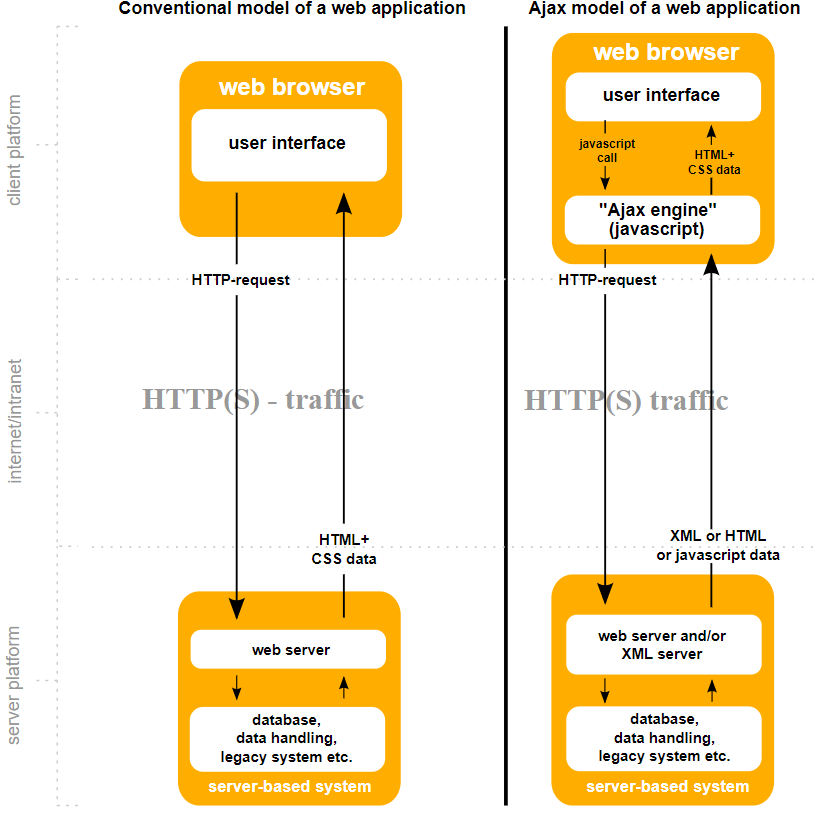
\includegraphics[width=\textwidth/2]{obrazky-figures/AJAX.png}
\caption{Konvenčí model pro webovou aplikaci versus aplikace používající AJAX.}
\end{figure}
\FloatBarrier

Na obrázku \ref{AJAX} je patrný rozdíl v komunikaci webové aplikace v konvenčním modelu ve srovnání s modelem používajícím AJAX. HTTP dotaz vytvoří přímo uživatel kliknutím, ale nejdříve je kontaktována AJAX logika běžící na pozadí pomocí JavaScriptu a teprve ta zašle HTTP dotaz. Jelikož není nutné čekat na získání odpovědi od serveru, je možné dále s webovou aplikací pracovat. V praxi ale uživatel získá odpověď téměř okamžitě.

        \subsection{Webové API}
Webové API (Application Programming interface) je rozhraní pro zpracovávání požadavků přes internet. Aplikace pošle požadavek, ten je následně zpracováván mimo aplikaci a po dokončení je aplikaci zasláno zpětné volání. Webové API mohou být AJAX dotazy na server nebo na databázi, může se jednat také o API prohlížeče jako je například odpočet času a podobně. Při zpětném volání je zaslán také objekt s odpovědí, a to nejčastěji ve formátech JSON a XML. API nepotřebují vědět, jaká aplikace je volá, potřebují znát pouze požadavek, který předají ve formátu definovaném v požadavku. Tento přístup je velmi podobný třídám s metodami v objektově orientovaném programování \cite{webapis}.
        \subsection{JQuery}
JQuery je volně dostupnou knihovnou, která zakomponovává více technologií, které zjednodušují práci s JavaScriptem. Známý slogan této knihovny, který ji současně i dobře vystihuje, je “Write less, do more” neboli “piš méně, udělej více”. Pro JavaScript zajistila jQuery zjednodušenou selekci a práci s DOM, DOM manipulaci pomocí CSS atributů a animace elementů a její součástí je také AJAX. Především tato knihovna ale zajišťuje kompatibilitu napříč prohlížeči. Každý prohlížeč zpracovával JavaScript vlastním způsobem, značné množství příkazů tak bylo nutné uzpůsobit pro prohlížeč, což byla jedna z největších kritik JavaScriptu. JQuery většinu s tím spojených problémů umí řešit, jelikož příkazy, které obsahuje, jsou vnitřně přeložené tak, aby jim prohlížeč rozuměl. Pro jQuery byla sepsána kvalitní dokumentace a stojí za ní velká komunita programátorů, zároveň se tato knihovna stala tak populární a revoluční, že je považována téměř za aplikační rámec.
Tabulka X. Srovnání zápisu základních příkazů v JavaScriptu a jQuery \cite{jquerybook}.

\FloatBarrier
\begin{table}[h!]
  \begin{left}
    \caption{Srovnání zápisu základních příkazů v JavaScriptu a jQuery}
    \label{tab:table1}
    \resizebox{\textwidth}{!}{
    \begin{tabular}{l|l}
      \textbf{JavaScript} & \textbf{jQuery}\\
      \hline
      document.querySelectorAll(‘.test-Class’) & \$(‘.test-Class’);\\\hline
      
      document.getElementById(‘#test-Id’).style.display = “none”; & \$(‘.test-Id’).hide();\\\hline
      
      \begin{tabular}{@{}l@{}}
      var h1 = document.CreateElement(“h1”); \\
      h1.innerHTML = “Nadpis”;\\
      document.getElementsByTagName(‘body’)[0].appendChild(h1);
      \end{tabular} & \$(‘body’).append(\$(“<h1/>”).html(“Nadpis”))\\\hline
      
      \begin{tabular}{@{}l@{}}
      var el= document.getElementById(‘test’);\\
      el.addEventListener('click', function() \{\\
      alert('TEST”');\\
      \}, false);
      \end{tabular} & 
      \begin{tabular}{@{}l@{}}
     \$(‘#test’).click(function() \{\\
      alert('TEST”');\\
      \});
      \end{tabular}\\\hline
     \end{tabular}}
  \end{left}
\end{table}
\FloatBarrier
Zápis v jQuery je oproti JavaScriptu zpravidla výrazně kratší a přehlednější (viz tabulku \ref{tab:table1}). Mnoho vlastností jQuery bylo postupem času integrováno do JavaScriptu. Podle W3Techs je jQuery používáno v 95 \% webových stránek používající JavaScript \cite{w3techs}.
        \subsection{Node.js}
Volně dostupné programovací prostředí (run-time) pro JavaScript s názvem Node.js umožňuje spouštět JavaScript mimo webový prohlížeč. Node.js byl postaven na Google V8 JavaScript jádře a byl navržen pro tvorbu škálovatelných síťových aplikací. Node.js obsahuje vestavěnou knihovnu, která umožňuje aplikacím fungovat jako webový server. Díky této technologii je možné používat JavaScript podobně jako jazyk PHP na serverové části aplikace. Node.js funguje na principu událostmi řízeném přístupu a v kombinaci s I/O API s neblokujícím přístupem, která optimalizuje přijímání a odesílání dat, umožňuje Node.js komunikaci mezi klienty a serverem v reálném čase. Node.js čeká na webovém portu na požadavky od uživatelů, po zachycení je požadavek vložen do jednovláknové smyčky událostí (event loop). Následuje zpracovávání požadavku, během něhož jsou zachytávány a zpracovávány další požadavky, které běží asynchronně na vlastních vláknech. Jednodušší požadavky tak mohou být zpracovávány rychleji.Celý proces zpracovávání požadavků je následující:
\begin{enumerate}
  \item Node.js získá požadavek od klienta.
  \item Požadavek je vložen do smyčky událostí, která je dále rozřazuje pro zpracování. Pokud příchozí požadavek není možné zpracovat, je vložen do fronty událostí.
  \item Požadavek je postupně zpracováván rozdělením na podúlohy. Pokud je možné úlohu zpracovat okamžitě nebo asynchronně(nebude tedy blokovat I/O), bude zpracována. Pokud se ale jedná o úlohu, která je synchronní, je předána některému z C++ vláken, které na něm dále pracují.
  \item Smyčka událostí je upozorněna dokončenou úlohou pomocí zpětného volání.
  \item Smyčka buď čeká na vyřízení jiné úlohy daného požadavku, nebo požadavek dokončí.
\end{enumerate}
Node.js exceluje při zpracovávání většího množství malých celků dat, tyto úlohy zpracovává s minimální odezvou \cite{nodejsevent}. Problém nastává pouze při provádění velkých výpočtů, které zaneprázdní všechna vlákna přidělená pro Node.js. V praxi je mnohem častější práce s malými výpočty, tudíž je tato nevýhoda velmi specifická a v kontrastu s výhodami je v běžném použití zanedbatelná. Jedná se také o relativně novou technologii, takže nativně podporuje moderní technologie jako například NoSQL databáze. Většina projektů vytvořených pomocí Node.js jsou zaindexované v registrech npm, tudíž se dají snadno dohledat a využít jako komponenty v aplikacích. Komunita spojená s Node.js se rychle rozrůstá, což podporuje zvyšování efektivity práce programátorů \cite{nodejsdevelopment}.

Společnosti jako jsou PayPal, Netflix, eBay převedly své webové aplikace na Node.js a zaznamenaly rychlejší vývoj aplikace, kratší vývojovou dobu a v některých případech menší počet lidí potřebných na vytvoření aplikace. Tato technologie také umožňuje snadné osvojení jazyka, JavaScript je totiž jeden z nejzákladnějších jazyků pro tvorbu na webu, a tak je přechod na serverovou logiku jednodušší. Komunikace mezi klientem a serverem probíhá ve stejném jazyku, což usnadňuje její přehlednost.

        \subsection{Npm}
Npm neboli Node Package Manager byl vytvořen pro správu balíčků k Node.js za účelem snadného sdílení, verzování a implementování kódu. Později se pak ale stal správcem všech javascriptových balíčků. V roce 2017 obsahoval 350 000 balíčků, čímž se stal největší kolekcí kódu v jednom jazyce. Npm se skládá z webové stránky, kterou lze využít pro objevování potřebných balíčků, Command Line Interface (CLI) neboli příkazového řádku, který běží v terminálu a umožňuje integrovat npm registr s obrovskou databází javascriptového softwaru a meta-informací s nimi spojenými. Základním úkolem balíčků je řešit konkrétní problémy nebo požadavky použitím cizího řešení tohoto problému. Často se přitom jedná o řešení osob kvalifikovanějších na danou problematiku. Balíčky by neměly řešit několik různých problémů naráz, ale měly by být definované pro specifickou potřebu. Díky tomu totiž vzníká modulární způsob programování, který podporuje systém vzájemného sdílení těchto modulů mezi programátory. Pokud nebude nalezeno potřebné řešení pro problematiku, může programátor implementovat vlastní a opět jej sdílet s ostatními. Balíčky mívají často podporu tvůrce či tvůrců a ostatní mohou navrhovat úpravy pro lepší implementaci. Idea nepsat kód, který už byl napsán mnohokrát předtím umožňuje rychlejší vývoj generických částí aplikace, jako je například přihlašovací formulář, navigace na stránce, tabulky apod. Tyto aplikační objekty je navíc možné převzít od předních a specializovaných vývojářů \cite{npmdocs}. 
        \subsection{TypeScript}
TypeScript je stručně řečeno rozšířenou verzí JavaScriptu. JavaScript totiž nikdy nebyl vytvořen k tomu, aby spravoval serverovou část aplikace, a proto mu chybí jisté prvky typické pro takové jazyky. Hlavní rozdílem je to, že JavaScript je čistě skriptovací jazyk. Dalším rozdílem je typování funkcí a proměnných, které podporuje strukturu kódu. TypeScript byl vytvořen, aby řešil právě tyto nedostatky. Jedná se o rozšíření jazyka JavaScript se zaměřením obohatit JavaScript o pravidla usnadňující programování aplikační logiky. TypeScript je silně typovaný, objektově orientovaný, kompilovaný jazyk. Kód v Typescriptu je při použití přeložen kompilátorem do čistého JavaScriptu. Jedná se tedy prakticky o maketu udržující strukturu kódu, která obsahuje několik prvků pro podporu vývoje kompletních webových aplikací. TypeScript je s JavaScriptem kompatibilní do takové míry, že pro konvertování javascriptového kódu do typescriptového stačí změnit koncovku souboru z .js na .ts. 

Díky podobnosti je veškerý kód JavaScriptu spustitelný v jazyce TypeScript, a tudíž i všechny knihovny JavaScriptu. TypeScript je navíc podporován na všech platformách, kde je spustitelný JavaScript - je tak podporována i veškerá infrastruktura a systém vzájemného sdílení kódu pomocí komponent či knihoven. Také run-time prostředí podporující JavaScript podporuje i typescript. Typescript navíc upozorňuje na chyby nalezené při kompilaci do JavaScriptu, což ulehčuje hledání chyb a jejich opravu \cite{typescriptweb}.

        \subsection{Webové komponenty}
Webové komponenty jsou sada technologií, které umožňují vytvářet vlastní znovupoužitelné webové prvky, které obsahují veškerou funkcionalitu zapouzdřenou a tím oddělenou od zbytku kódu. Tyto prvky je pak možné používat napříč aplikací bez vzniku konfliktů. Jedná se tedy správnou metodiku v rámci programování, která je aplikovatelná na celé aplikace. Webové komponenty se skládají ze tří technologií. Technologie vlastně vytvořených webových prvků, jedná se o rozhraní API JavaScriptu, které umožňuje definovat vlastní prvky a jejich chování. Další technologie je Shadow DOM, jedná se o několik API JavaScriptu pro připojení stínového stromu DOM k prvku. Tento DOM se vykresluje odděleně od hlavního stromu DOM aplikace. Dále se k prvku připojí ovládání zapouzdřených funkcí. Funkcionalita prvku je tedy naprosto oddělena od funkcionality aplikace ve které je prvek vložen. Poslední technologií jsou HTML šablony, šablony se značí <template> tyto umožňují psát šablony které nejsou zobrazené na stránce, ale pořád určují strukturu komponenty \cite{webcomponentsaction}.
  \chapter{Javascriptové aplikační rámce}
Nejpodstatnější technologií spojenou s JavaScriptem jsou ale aplikační rámce neboli frameworky. Tyto aplikační rámce v sobě spojují dříve popisované technologie a navíc přidávají mnoho dalších funkcí, které usnadňují tvorbu aplikací. Javascriptové aplikační rámce jsou nezbytnou součástí moderního webového vývoje front-end, neboli prezenční část aplikace běžící na straně klienta, a poskytují vývojářům osvědčené nástroje pro vytváření škálovatelných interaktivních webových aplikací. Rámce jsou typem nástroje, díky kterému je práce s JavaScriptem jednodušší a plynulejší. V jejich nejzákladnějším prostředí jsou rámce kolekcí knihoven kódů JavaScriptu, které vývojářům poskytují předem napsaný kód, který lze použít pro rutinní programovací funkce a úkoly - tedy doslovně rámec pro vytváření webů nebo webových aplikací. 

Výhoda v používání aplikačních rámců JavaScriptu je celková efektivita a organizovanost, které do projektu přinášejí. Frameworky často obsahují efektivnější a bezpečnější implementace některých funkcí jako je například bezpečné ukládání dat a efektivní užití knihoven. Kromě toho rámce navádějí na přehledné strukturování kódu a poskytují hotová řešení pro běžné problémy s kódováním. Na druhou stranu může být celá tato struktura nevýhodou v tom, že vyžaduje dodržování pravidel a konvencí specifických pro daný framework, což omezuje svobodu, kterou programátorovi nabízí úplně ruční kódování. Částečnou volnost při strukturování projektu nabízí využití knihoven, které rovněž obsahují velké množství předdefinovaných technologií. Rozdíl mezi knihovnou a aplikačním rámcem je tedy to, že aplikační rámec má přesně definovanou strukturu, kterou se vývojář musí řídit, a obsahuje téměř veškeré technologie potřebné pro úplný vývoj aplikace včetně sestavování aplikace, jejího testování, vytváření síťových požadavků apod. Knihovny také nabízí tyto nástroje, ale jejich využití je často podmíněno použitím knihoven a komponent třetích stran. Knihovny nemají striktní pravidla pro strukturu aplikace a použití nabízených technologií je zcela volitelné.

Podrobnější informace ohledně tří nejpopulárnějších javascriptových aplikačních rámců budou představeny v následujících podkapitolách. Jedná se konkrétně o Angular, Vue a React, přičemž rámci React se budu věnovat pouze stručně, jelikož ve své práci se zaměřuji především na srovnání Angularu a Vue \cite{clientsideframe}.

    \section{Angular}
Prvním javascriptovým aplikačním rámcem, kterému zde bude věnována pozornost, je Angular. Jedná se o aplikační rámec vytvořený společností Google v roce 2016. Před touto verzí existoval Angular.js, který byl ve všech aspektech komplikovanější verzí stávajícího Angularu. Angular je plnohodnotný aplikační rámec, což znamená, že obsahuje veškeré technologie potřebné pro sestavení plně funkční aplikace, má jasně definovanou architekturu a obsahuje i nástroje pro testování aplikace. Rámec Angular využívá technologii RxJS umožňující pracovat s datovými toky, které obsahují asynchronní data, tyto data se mohou dynamicky měnit v reálném čase. V Angularu jsou definována jako pozorovatelné proměnné neboli observables a dají se filtrovat, mapovat a zpracovávat. Tato data mohou být závislá na třetí straně, která je ve chvíli změny, předá aplikaci k dalšímu zpracování. Pozorovatelné proměnné tak v danou chvíli nemusí být nutně součástí kódu, ale ve chvíli, kdy začnou existovat, spustí se předem definované procesy \cite{angularforenterprise}.

Angular používá pro předlohu jazyk HTML a pro veškerou vnitřní logiku využívá TypeScript, přičemž TypeScipt je kompilován do čistého JavaScriptu. Šablona je převážně napsána v HTML a přijímá téměř všechny značky HTML až na značku “<script>”. Tato značka je ignorována, aby nedocházelo k vkládání cizího kódu a ke zneužití aplikace. Angular umožňuje zobrazení dat v šabloně pomocí dvojitých složených závorek {{data}}.

Rámec Angular podporuje obousměrnou datovou vazbu, což je mechanismus pro komunikaci šablony s komponenční logikou a naopak. Tato komunikace může být obousměrná, ale i jednosměrná pro obě varianty. 

Angular dále používá inkrementální DOM pro aktualizaci náhledů. Všechny komponenty projdou kompilací, neboli převedením do setů instrukcí. Tyto instrukce jsou poté použity pro vytvoření DOM stromu, sady instrukcí jsou následně porovnány a rozdíly jsou upraveny podle potřeby. Popisovaná DOM struktura díky kompilaci umožňuje proces zpracování zvaný tree-shaking, který u virtuálních DOM struktur není možný. Tree-shaking je proces, kdy se zkontroluje, zda jsou vygenerované instrukce využity a pokud nejsou, jsou během kompilace smazány. Díky tomu, že není nutné generovat virtuální DOM, jako je tomu u ostatních aplikačních rámců, šetří Angular místo v paměti a ve spojení s procesem tree-shaking zajišťuje, že je použito minimální množství paměti. Tato vlastnost je velmi výhodná při použití na mobilních aplikacích Problematické je však to, že se tím prodlužuje kompilační doba náhledu. 

Architektura Angular aplikace se opírá o určité elementární koncepty. Základními stavebními bloky aplikačního rámce Angular jsou komponenty neboli components. Tyto komponenty jsou poté organizovány do modulů NgModules. Moduly shromažďují související kód do sad plnících určitou funkci. Angular aplikace je pak definována skupinou těchto modulů. Aplikace má vždy kořenový modul, který umožňuje sestavení aplikace. Kořenový modul je běžně pojmenován AppModule a poskytuje mechanismus bootstrap, který aplikaci inicializuje a spouští. Tento modul může také obsahovat neomezenou hierarchii podřízených modulů. Moduly jsou často organizovány do logických celků pro větší přehlednost při vývoji větší aplikace \cite{angularforenterprise}.

Komponenty definují a spravují pohledy, což jsou skupiny elementů určené pro zobrazení, ze kterých si Angular může vybírat a upravovat je podle logiky a dat programu. Hlavní struktura pohledu je definována v šablonách. Šablony jsou většinou odděleny od samotné komponentové logiky a jsou umístěny do stejnojmenných souborů s koncovkou “.html”.
Komponenty používají služby (services), které poskytují konkrétní funkce, které přímo nesouvisí s pohledy. Mnohdy jsou to tedy obecné nástroje pro zpracování dat, které mohou být použitelné i v jiných komponentách. Tyto služby mohou být vloženy do libovolného počtu komponent. Kód je díky tomu modulární, opakovaně použitelný a efektivní. Moduly, komponenty a služby jsou třídy, které používají dekorátory. Tyto dekorátory určují jejich typ a poskytují potřebná metadata pro zpracování Angularem.

Každá komponenta má jakýsi životní cyklus, který se skládá z fází, ve kterých se dá s komponentou manipulovat. První ovlivnitelná fáze nastává před samotnou inicializací, používá se na k tomu hák ngOnChanges, který se provede před inicializací a poté rovněž vždy, když dojde ke změně některých dat. Poté přichází inicializace ngOnInit - tento hák se provede při samotné inicializaci. Po každé změně je spuštěn ngDoCheck, který slouží k zachycení změn, které Angular nemusí zaznamenat. Po inicializaci a vedlejší kontrole přichází inicializace obsahu ngAfterContentInit a jeho kontrola prostřednictvím háku ngAfterContentChecked. V tomto bodě dochází ke spuštění inicializace vnořených komponent. Dále po úplné inicializaci náhledů jak kontrolovaných komponent, tak komponent vnořených, je možné se připojit s hákem ngAfterViewInit a jeho kontrolou ngAfterViewChecked. Tímto je inicializace dokončena. Pokud jsou data změněna, přichází znovu inicializace a její kontroly a inicializace vnořených komponent. Jakmile už komponentu není potřeba dále vykreslovat, nastává fáze, během níž je komponenta a všechny vazby s ní spojené (například sledované proměnné, vnořené komponenty apod.) smazána a zde se dá navázat pomocí háku ngOnDestroy \cite{angularforenterprise}.

    \section{Vue.js}
Dalším aplikačním rámce JavaScriptu, který zde popíši, je Vue.js. Jedná se o technologii, která má zachovány podobnosti s rámcem Angular, ale blíží se také knihovně React, je to tedy něco na pomezí obou. Vue.js může být využíván jako odlehčená knihovna, ale může být použit i jako plně funkční aplikační rámec. Vue vytvořil Evan You, který se před prací na Vue podílel na vývoji Angularu. Angular považoval za příliš komplexní, ale viděl potenciál v některých jeho vlastnostech, rozhodl se proto extrahovat části, které na Angularu nejvíce doceňoval, a vytvořil z nich lehkou knihovnu. Ačkoli You zahájil tvorbu Vue při práci s Angularem, považuje Vue za nejpodobnější s knihovnou React, protože jeho základní myšlenkou je datová vazba a komponenty, což je základní funkcí Reactu. Architektura Vue se zaměřuje na vyobrazení náhledů a strukturu tvořenou z komponent s vlastními instancemi Vue. Vue je sám o sobě velmi jednoduše rozšiřitelný, a tak se hodí na tvorbu škálovatelných aplikací. Základní knihovna Vue se zaměřuje pouze na zobrazovací vrstvu, ale ostatní rámcové nástroje jsou v oficiálně udržovaných knihovnách a balíčcích jako je například Vue Router pro přesměrovávání v rámci aplikace nebo balíček Vue Server Render, který umožňuje generování Vue na serveru \cite{vuejsup}. 

Syntaxe Vue.js funguje na principu použití předloh v HTML jazyce, na kterou se navazuje skriptová část v JavaScriptu obsahující metody, data apod. Tyto dvě vrstvy jsou vzájemně propojené a komunikují spolu.. Data definovaná v javascriptové části aplikace lze vázat do HTML pomocí dvojité složené závorky podobně jako v Angular, tedy {{data}}.

Data komponenty jsou uloženy ve specializované funkci “data”, která vrací tato data jako anonymní funkce. Data mohou být mezi komponentami přeposílána za pomoci specializovaného objeku “props”. Každá takto předaná hodnota se stává novou instancí té hodnoty. S takto předanou hodnotou se dá pracovat stejně jako s hodnotou definovanou v “data” funkci.

Architektura aplikace Vue je tvořena komponentami, kdy každá komponenta reprezentuje vlastní instanci Vue. Každá komponenta musí obsahovat předlohu HTML a každá předloha se skládá z pouze jednoho kořenového elementu, uvnitř kterého je obsažen zbytek předlohy. Díky tomu je každá komponenta znovupoužitelná. Každá komponenta a tedy i instance Vue přijímá stejné vlastnosti (například data, zpracované hodnoty, metody a hákování na životní cyklus instance). Jedinou výjimkou je prvotní instance Vue, kterou je takzvaný “root” - tato instance má více možností jako například “el”, která odkazuje na kořenový element v DOM. Veškeré komponenty musí být zaregistrovány buď globálně, nebo lokálně. Vue aplikace se často skládá ze stromu obsahujícího komponenty, přičemž tyto komponenty se mohou znovu používat a zanořovat \cite{vuejsup}.

Vue oproti Angularu využívá virtuální DOM pro aktualizaci stránky. Vue se po sestavení předlohy připojí k DOM a sleduje vlastní data za účelem detekce případné změny. Pokud se hodnoty změní, Vue zpracuje koponentu a promítne ji na virtuální DOM. Poté srovná předchozí virtuální DOM s novým a změnu aplikuje na reálný DOM \cite{vuejsup}. Během tohoto procesu dochází k jistým fázím, které se nazývají životní cyklus, a Vue umožňuje dělat úpravy v daných fázích za pomoci hákování na tyto události v životním cyklu. Před vytvořením nové instance Vue je možné využít hák beforeCreate, který provede kód před vytvořením instance. Vue po dokončení tvorby instance zkontroluje, zda je nastaven příznak “el”. Pokud tomu tak je, pokračuje systém dále ve zpracovávání. Jestliže tomu tak není, bude instance Vue navázaná na rodičovský HTML element. Následně je zpracována HTML předloha. Dalším krokem je připojení instance k DOM, přičemž před provedením připojení je možné zavolat hák beforeMount a po připojení hák Mounted. Dále se pak opakovaně provádí kontrola dat, pokud předtím proběhly nějaké změny, a je možné se navázat na událost pomocí háku beforeUpdate. Dalším krokem je aktualizace virtuálního DOM a je možné se navázat skrze hák Update. Tento proces se opakuje do zavolání destruktora instance. Před samotným smazáním instance je možně použít beforeDestroy a po smazání instance se lze navázat hákem Destroyed \cite{vuelifecycle}.

    \section{React}
React nebo také ReactJS je v podstatě pouze javascriptová knihovna sloužící k vytváření frontendu webové aplikace. Je velmi odlišný od Angularu svou rozsáhlostí a komplexností. React byl vytvořen společností Facebook v roce 2013 jako reakce na rostoucí význam internetových reklam. Facebook chtěl mít k dispozici nástroj k jednoduššímu managementu těchto reklam. Podobně jako v případě jQuery se nejedná o framework, ale o velmi rozsáhlou knihovnu, která obsahuje takové množství technologií, že její používání významně ovlivňuje strukturu aplikace, čímž se podobá aplikačnímu rámci. React se vyznačuje tím, že jsou jeho konečná řešení rychlá, do určité míry jednoduchá a velmi jednoduše rozšiřitelná. Knihovnu React lze také přidat do existujícího projektu napsaného pomocí jiného nástroje. 

React obsahuje velké množství podpůrných knihoven umožňujících snazší vývoj aplikace. Zaměřuje se ovšem pouze na prezenční vrstvu aplikace, tudíž je při tvorbě s využitím Reactu nutné doplnit knihovny od třetích stran (například pro navigování nebo získávání dat). React slouží nejlépe k tomu, k čemu byl navržen, a je proto velmi simplistický a efektivní v modelování a práci s náhledy aplikace. Oproti Vue a Angularu si React zakládá na spojení náhledové logiky a samotného HTML. Pro usnadnění takového splynutí React přináší novou technologii rozšiřující JavaScript, a sice JSX. JSX je zkratka pro JavaScript XML. Jedná se o syntaktické rozšíření JavaScriptu. Konečným produktem JSX jsou prvky, které nejsou ani řetězci, ani součástí kódu HTML, ale kombinací obou. K libovolné proměnné tedy můžeme přiřadit hodnotu, která obsahuje prvky HTML. Pak React zajistí, aby tyto proměnné nebo části kódu byly aplikovány na DOM \cite{reactintro}.

Hlavním stavebním blokem aplikačního rámce React je komponenta. React využívá virtuální DOM, díky čemuž je upravena jen potřebná část stromu DOM. Každá komponenta je buď funkce, nebo třída, která musí obsahovat metodu vykreslení. Komponenty mohou přebírat data z rodičovské komponenty a tato data jsou uložena v objektu “props” a nelze je upravovat. Komponenta dále obsahuje objekt obsahující stav komponenty zvaný “state”. Pokud je tento stav změněn, dojde k opakovanému vykreslení komponenty. Data v Reactu jsou narozdíl od Angularu vázána pouze jedním směrem, tedy že logika kódu ovlivňuje náhled ale ne naopak. Aby proběhla změna opačným směrem, musí nastat událost (například kliknutí na tlačítko). Podobným způsobem jsou zpracována data předaná mezi komponentami - tedy vždy jen z nadřazené komponenty do vnořené komponenty. Pro zpětnou komunikaci je možné využít zpětného volání funkce předaného v parametrech komponenty \cite{reacttutorial}. V rámci Reactu není potřeba mluvit o životním cyklu aplikace, protože není používán. Proces vykreslování komponent je podobný jako ve Vue.

  \chapter{Výzkumný záměr}
Javascriptové aplikační rámce jsou v dnešní době při tvorbě webových aplikací čím dál častěji využívány. V rámci JavaScriptu jsou aplikační rámce nejvlivnější technologií a poptávka po vývojářích, kteří s nimi umí pracovat, je vysoká. Aplikace mají díky nim stabilnější strukturu, jsou bezpečnější, modulárnější a dají se snadno škálovat. Díky své obsáhlosti umožňují aplikační rámce velmi rychlý vývoj aplikací. Dříve představené javascriptové aplikační rámce naplňují podobné úkoly, ale v mnoha vlastnostech se od sebe liší, proto je podstatné je srovnat a vymezit jejich použití. Každý rámec se hodí pro jiné účely, některé jsou například vhodnější pro tvorbu menších aplikací a jiné jsou ideální pro tvorbu aplikací zaměřených na grafiku anebo pro aplikace s rozsáhlou systémovou logikou. V této práci je mým záměrem srovnat dva ze dvou popsaných rámců, konkrétně se jedná Angular a Vue.

Jedním ze způsobů, jak je možné oba aplikační rámce srovnat, je vytvoření aplikace, v níž by bylo možné vidět potenciál popisovaných technologií a rozdíly mezi nimi. Taková aplikace by měla být natolik komplexní, aby její vnitřní logika byla rozsáhlá a aby mohla mít i reálné využití. Jednoduchá testovací aplikace by neumožnila takovou míru srovnání v kritériích, na které se chci zaměřit. Výzkumy využívající totožné testovací aplikace v různých aplikačních rámcích a porovnávající charakteristiky jako je například rychlost zpracování, velikost výsledného souboru ap. navíc již existují. Cílem této práce je však srovnat špatně kvantifikovatelné rozdíly, které jsou spojeny s praktickým a cíleným využitím aplikačních rámců. Na základě poznatků vyplývajících z literární rešerše jsem se rozhodl využít jako hlavní aplikační rámec Angular doplněný o komponenty vytvořené pomocí rámce Vue. Angular je určený pro mohutnější aplikace, má stabilnější architekturu a má v sobě implementovanou jednoduchou komunikaci se serverem pro případnou práci s databází. Vue je narozdíl od toho odlehčený aplikační rámec, který je lehký a rychlý, a bývá běžně využíván k tvorbě univerzálně využitelných komponent.

Pro účely takového srovnání jsem se rozhodl navrhnout a vytvořit webovou aplikaci umožňující správu a prodej lístků na události. Tato aplikace bude rozdělena do tří částí, kterými jsou prodej vstupenek, správa vstupenek a kontrola vstupenek. Prodej vstupenek bude zobrazovat aktuální počet volných vstupenek preferovaně v reálném čase, jeho součástí bude platební brána a funkce umožňující poslat vstupenku uživateli anebo mu ji zobrazit. Správa vstupenek pak bude obsahovat minimálně seznam událostí, na které je možné zakoupit vstupenky, a formulář pro tvorbu nových událostí nebo jejich úpravu či smazání. Část sloužící ke kontrole vstupenek bude přijímat kódy vstupenek. K tomuto bude využita technologie načítání QR kódů a následné zobrazení, zda je vstupenka platná či ne.
 
  \chapter{Popis aplikace}
V této kapitole popisuji implementaci dříve navrhnuté webové aplikace. Je vhodné upozornit, že popis je v mnohém spíše zjednodušený, a to z toho důvodu, že je celá aplikace komplexní a obsáhlá. Pro účely této práce považuji detailnější popis aplikace za přebytečný. Celý kód nicméně obsahuje komentáře, které umožňují porozumění jednotlivým částem. 
Aplikace je pojmenována Ticketeer neboli Vstupenkovač. Je rozdělena do následujících částí: prodej vstupenek, správa vstupenek, kontrola a nakonec vizualizace vstupenek. Do těchto částí rozdělím pro větší přehlednost textu také popis této aplikace.

Hlavní část aplikace je napsána pomocí aplikačního rámce Angular. Angular se stará o veškerou aplikační logiku jako je rozpoznání uživatele, komunikace s databází, zpracování formulářů pro události, vytvoření tabulky pro náhled aplikace, použití platební brány, zaslání vstupenky e-mailem, kontrola vstupenky a veškerá komunikace mezi komponentami aplikace.

Aplikační rámec Vue byl využit pro grafické generování samotných vstupenek a jejich převedení do souborové podoby. Vstupenky jsou generovány na základě předlohy, která obsahuje unikátní QR kód, a jsou nabídnuty ke stažení. Jejich kopie je také zaslána na zadanou e-mailovou adresu.

Veškerá komunikace s databází a kontrola oprávnění je vytvořena za pomoci pozorovatelných datových toků neboli “observables”. Tento přístup zajišťuje získávání dat v reálném čase s minimální zátěží sítě, klienta i serveru. Většina procesů se odehrává na straně klienta. Aplikace se typově řadí mezi single-page aplikace (SPA), což znamená, že uživatel není nikdy přesměrován na jinou stránku, ale dochází podle potřeby ke změnám náhledů. Data a procesy na straně klienta jsou zabezpečeny, aby nebylo možné je zneužít. Výsledná aplikace sestává ze dvou vygenerovaných značek HTML v podobě webových komponent. Tyto komponenty obsahují celou aplikace za účelem možnosti použití aplikace na libovolné webové stránce. Uvnitř jedné z těchto webových komponent se nachází webová komponenta vytvořená v aplikačním rámci Vue.

    \section{Použité technologie}
Aplikace byla napsána za použití programovacího integrovaného vývojové prostředí IntelliJ IDEA. Toto prostředí bylo navrženo pro vývoj aplikací v jazycích Java a JavaScript, tudíž obsahuje podpůrné nástroje pro psaní kódu za pomoci javascriptových aplikačních rámců. Obsahuje podporu pro našeptávání kódu, která zobrazuje návrhy na základě existujících názvů, funkcí, knihoven apod. Během psaní ověřuje, zda jsou typy proměnných odpovídající pro dané použití. IntelliJ IDEA také pomáhá s hromadným přejmenováním napříč soubory. Upozorňuje na duplicitní kód a umožńuje rychlé zobrazení definice funkce nebo proměnné a jejich výskytu napříč projektem. Dále umožňuje debugging uvnitř kódu, spojení s verzovacím systémem Git a jeho grafickou vizualizaci a další pomocné nástroje usnadňující vývoj aplikace \cite{intellijidea}.

Aplikace byla během vývoje verzována a ukládána pomocí nástroje Git na webové úložiště. Díky tomu bylo možné vracet se na předchozí verze aplikace a rozdělovat práci do několika odvětví, která na sobě nebyla závislá a při nedokončení implementace jedné větve umožňovala, aby byl kód na ostatních větvích bez chybových hlášek \cite{gitreference}.

Pro úvodní inicializaci projektu a jeho rozšiřování o komponenty a volně dostupné balíčky byl použit nástroj Angular CLI. Jedná se o rozhraní v podobě příkazového řádku, které přidává do terminálu možnost použít příkazy, které například generují soubory se všemi potřebnými konfiguracemi, umí spustit aplikaci na lokálním serveru apod. Přes tyto příkazy je možné snadno sestavit aplikaci do produkční podoby, což zajišťuje, že se programátor může věnovat pouze vývoji a nemusí se zabývat mechanikami aplikačního rámce.

Pro správu balíčků byl vybrán dříve zmiňovaný npm. Npm je oproti svým konkurentům obsáhlejší, populárnější a obsahuje systém upozorňující na části kódu, které jsou zranitelné ve smyslu bezpečnosti. Balíček nainstalovaný pomocí npm automaticky doplní závislosti a zajišťuje stahování aktuálních verzí balíčku. Tento nástroj značně ulehčuje použití modulů třetích stran.

    \section{Databáze}
Aplikace využívá databázi a online hostování funkcí na platformě Firebase. Jedná se o platformu vytvořenou společností Google pro tvorbu mobilních a webových aplikací. Firebase je jádrem prezentované aplikace. Firebase nabízí vývojáři nespočet nástrojů pro tvorbu aplikací, jako je například databáze odpovídající v reálném čase, hostování webu, cloudové úložiště, autentizace, cloudové funkce, vzdálenou konfiguraci aplikace, testování, monitorování komunikace. Firebase umožňuje vývojářům při vývoji aplikace bezplatně k těmto nástrojům přistupovat, nepřekročí-li určité limity. Pokud vytvořená aplikace nedosahuje výrazného provozu, je možné tuto platformu bezplatně využívat i nadále.

Firebase nabízí mnoho variací NoSQL databází. Pro tento projekt je použita varianta Cloud Firestore. Databáze NoSQL poskytuje mechanismus pro ukládání a načítání dat, který je modelován jinými způsoby než tradičními tabulkovými relacemi používanými v relačních databázích jako je SQL. Cloud Firestore je flexibilní škálovatelná cloudová databáze NoSQL, která umožňuje ukládat a synchronizovat data pro vývoj na straně klienta i serveru. Stejně jako Firebase databáze udržuje Cloud Firestore data synchronizovaná v reálném čase mezi klientskými aplikacemi, a to prostřednictvím posluchačů, a nabízí offline podporu pro mobilní zařízení a web. Je tak možné vytvářet responzivní aplikace, které fungují bez ohledu na odezvu sítě nebo připojení k internetu. Tato databáze se dá snadno spojit s cloudovými funkcemi na platformě Firebase.

Struktura databáze je rozdělena do kolekcí dokumentů obsahujících data. Na obrázku X lze vidět reprezentaci databázové hierarchie tak, jak se vyskytuje v aplikaci. Jelikož se jedná o NoSQL databázi, jsou relace mezi kolekcemi zcela deskriptivní.

\FloatBarrier
\begin{figure}[!htb]
\label{Database}
\centering
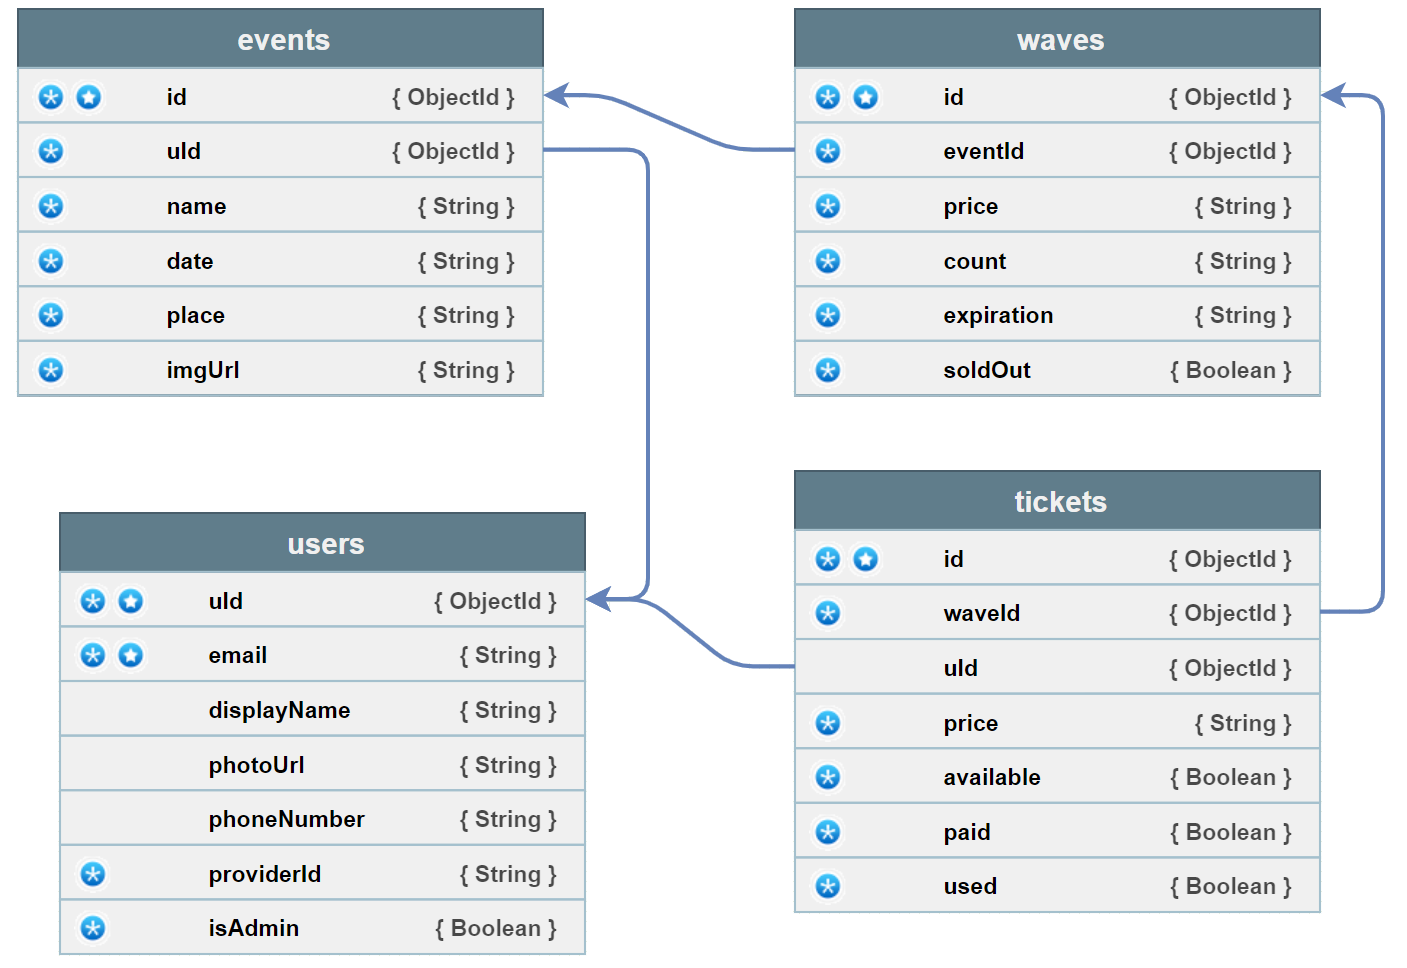
\includegraphics[width=\textwidth]{obrazky-figures/database.png}
\caption{Model databáze}
\end{figure}
\FloatBarrier

Databáze obsahuje dokumenty se strukturou strukturou vyobrazenou na obrázku \ref{Database}. V levé části každého z bloků je označení toho, zda je položka povinná (reprezentováno ikonkou s vločkou vlevo) a zda je unikátní (reprezentováno ikonkou s hvězdou vpravo). Dále je možné vidět název proměnné a ve složených závorkách je typ proměnné. ObjectId je typ unikátně vygenerovaného ID složeného ze znaků a číslic. Uživatel (user) má povinné unikátní ID a také unikátní e-mailovou adresu, pomocí které se po zadání hesla může přihlásit do systému. Následují volitelné položky jako zobrazované jméno (displayName), obrázek avatara uživatele (photoUrl) a telefonní číslo (phoneNumber). Tyto parametry jsou automaticky vygenerovány při přihlášení pomocí Google účtu. Zbývají dva další povinné parametry, a to způsob přihlášení uživatele (providerId), které může proběhnout pomocí Google účtu nebo přímou tvorbou účtu, a dále příznak udávající práva uživatele (isAdmin) přistupovat k vytváření vlastních událostí a ke kontrole vstupenek. 

Události (events) mají unikátní povinné id a povinné uId shodující se s ID tvůrce události. Každá událost má povinné jméno (name), datum konání (date), místo konání (place) a odkaz na grafickou předlohu pro vstupenku (imgUrl). Každá událost se skládá z vln, během kterých se prodávají vstupenky za různou cenu. Vlny vstupenek (waves) mají povinné unikátní id, dále mají eventId shodující se s id událostí, v rámci které se vlna nachází. Vlna vstupenky obsahuje povinné položky - cenu, za kterou se vstupenky prodávají (price), počet vstupenek ve vlně (count), datum kdy je prodej vlny ukončen (expiration) a příznak, zda je vlna vyprodána (soldOut). Vstupenky mají také unikátní povinné id a waveId shodné s id vlny, ke které se vstupenka váže. Následuje nepovinné id klienta, který vstupenku vlastní (uId). Každá vstupenka má povinně cenu (price) a příznaky jestli je vstupenka volná (available), zaplacená (paid) anebo použita (used).

    \section{Prodej vstupenek}
Prodej téměř celý probíhá v angularové části aplikace. Po příchodu na webovou aplikaci se zobrazí komponenta TicketComponent a při spuštění se načtou služby a data potřebné pro komunikaci s databází, pro spouštění funkcí na serveru a kontrolu uživatelských údajů. Celá logika prezentování obsahu je rozdělena do několika fází. Těmi jsou úvodní náhled, zakoupené vstupenky, autentizace, platební brána a úspěšné nebo neúspěšné zakoupení. Komponenta se spojí s databází Firebase a vyžádá si pozorování vstupenek s ID události, na které se vstupenky prodávají. Tento proces zajišťují funkce uvnitř dvou vlastně vytvořených služeb TicketService a Ticket EventService. Tyto služby zajišťují komunikaci mezi komponentami a databází za pomocí sledovatelných proměnných.

První fází je úvodní náhled, v rámci něj se v reálném čase na stránce zobrazuje počet volných vstupenek spolu s jejich cenou. Pro zakoupení vstupenky musí být uživatel přihlášen, tzn. po kliknutí tlačítka zakoupit vstupenku je zobrazen buď přihlašovací nebo registrační formulář. Samotná registrace a přihlašování se nachází ve fázi autentizace. Proces registrace a přihlašování je řízen za pomoci volně dostupné knihovny ngx-auth-firebase. Tato knihovna v sobě zakomponovává autentizaci pomocí Firebase a úhledně působící formulář k přihlášení a registraci.

Po přihlášení je uživatel vrácen na úvodní náhled a může zakoupit vstupenku nebo rozbalit menu. V menu se nachází možnost zobrazení zakoupených vstupenek a odhlášení. Zobrazení vstupenek je součástí komponenty naprogramované v rámci Vue, této části se tak budu věnovat později.

Kliknutím na tlačítko “koupit” vstupenku v reálném čase dojde k zarezervování vstupenky pro daného uživatele. Náhled se posléze změní na platební bránu, která byla implementována pomocí knihovny ngx-braintree. Tato knihovna zajišťuje přístup k platební bráně společnosti Braintree a předává informace jako je typ platby a měna, v níž transakce probíhá. Tato platební brána je známá především v zahraničí a nabízí kvalitní testovací prostředí. Zde se dostáváme k serverové logice, která je obsažena v souboru index.tx. Tento soubor obsahuje funkce napsané v Typescriptu, které běží na platformě Firebase. Nejdříve je zažádáno o token transakce pomocí požadavku na serverovou funkci hostovanou platformou Firebase. Ta zažádá webové rozhraní Braintree, aby předalo token, který je klíčový pro komunikaci během transakce. Jakmile je token získán, zobrazí se formulář pro platební údaje klienta. Po vyplnění údajů a stisknutí tlačítka “zaplatit” je spuštěna další serverová funkce, která zpracuje token a údaje uživatele a pošle je na rozhraní Braintree. Jsou-li údaje správné a transakce tak proběhne v pořádku, je skrze jinou serverovou funkci vygenerován PDF soubor se vstupenkou, který je pomocí služby SendGrid e-mailem zaslán na e-mailovou adresu klienta. Zároveň je uživatelem rezervovaná vstupenka v databázi označena jako zaplacená a je k ní přiřazeno ID uživatele. Pokud bude tento proces trvat déle než deset minut, bude uživatel přesměrován na úvodní náhled a rezervovaná vstupenka bude uvolněna k rezervaci dalšími uživateli.

Následně je uživatel přesměrován do poslední fáze, a to je úspěšné a nebo neúspěšné provedení transakce. Při neúspěšném provedení není vstupenka zaslána, její rezervace danému uživateli končí a uživatel je informován o neúspěšné transakci. Pokud proběhne úspěšně, je uživateli umožněno stažení PDF souboru se vstupenkou. V obou případech je uživateli zobrazena vytvořená animace SweetAlert a po je chvíli uživatel přesměrován zpět na úvodní náhled.

	\section{Správa vstupenek}
Správa vstupenek je vytvořena pouze za pomoci Angularu a je obsažena v komponentě AdminComponent. Po spuštění administrativní části aplikace je podobně jako u prodeje navázáno spojení s databází Firebase a nastane kontrola, zda je uživatel přihlášen a zda má právo vytvářet a spravovat vlastní události. Pokud uživatel není přihlášen, je mu předložen formulář pro přihlášení pomocí knihovny ngx-auth-firebase. Uživatel se může přihlásit pomocí Google účtu nebo účtu v aplikaci.

Po pokusu o přihlášení je v databázi zkontrolováno, zda má uživatel příznak administrátora. Pokud tomu tak není, přihlášení je neúspěšné a uživatel je upozorněn, že tato sekce je pouze pro administrátory. V případě, že se jedná o osobu s oprávněním, je uživatel přivítán a může pomocí tabulky sledovat prodej vstupenek na událost, upravovat události, spustit kontrolu vstupenek anebo vytvářet nové události.

Logika pro zobrazení tabulky je obsažena v komponentě TicketEventTable. Do této kompenty je zasláno ID přihlášeného uživatele. Komponenta současně obsahuje informace o rozložení tabulky. Pro umožnění plynulého dynamického generování tabulky, která je aktualizována při změnách v databázi, byla použita tabulková komponenta z UI knihovny Angular Material, ve spojením s hákem ngAfterViewInit. Knihovna Material vykreslí předdefinovanou strukturu tabulky úhledným a responzivním způsobem. Uvnitř háku ngAfterViewInit jsou změny dat zachyceny pomocí funkce obsažené ve službě TicketEventService. Data získaná pomocí služby TicketEventService jsou poté zpracována a převedena do formátu vhodného pro zobrazení pomocí Material tabulky. Tabulka obsahuje ID události, název, datum konání, tlačítka pro úpravu události a kontrolu vstupenek. Na řádek obsahující událost je možné kliknout, čímž se zobrazí detaily o vlnách události. Nachází se tam informace o tom, zda je vlna vyprodaná, datum expirace prodeje vstupenek vlny, cena vstupenek, celkový počet vstupenek a počet volných vstupenek. Kontrolou vstupenek se budu zaobírat v následující kapitole.

Tvorbu nebo úpravu události spravuje jedna komponenta, konkrétně CreateOrEditTicketEventDialog. Zpracování těchto požadavků se v jistých bodech liší, ale převážně prochází stejným postupem. Při tvorbě události se otevře modální okno s formulářem, kde jsou všechna pole povinná a obsahují typovou kontrolu. Formulář je v pozadí sestaven z několika komponent, které jsou založené na formulářích z rámce Angular a designu vstupních polí z knihovny Material. Textová a číselná pole jsou instance komponenty InputComponent, která zajišťuje ucelený vzhled, základní kontrolu hodnot a zobrazení chybové hlášky. Pole určená pro datum jsou instance DatepickerComponent. Tato komponenta umožňuje využití našeptávače dat implementovaného za pomoci knihovny Moment anebo malého okna zobrazujícího kalendář, který vychází z knihovny Material. Jestliže uživatel nezadal úplně datum a kliknul jinam, komponenta se pokusí doplnit chybějící informace. Například při pouhém zadání hodnoty “15” bude datum doplněno o aktuální měsíc a rok, aby formát odpovídal požadavkům. Dále byl implementován validátor, který dynamicky kontroluje, zda jsou data v logickém pořadí. Takto validátor znemožňuje, aby bylo zadáno datum konání akce, které by mělo proběhnout dříve než má být ukončen prodej vstupenek některé z vln. Aby fungovala komunikace mezi poli, všechny tyto komponenty jsou rozšířeny o abstraktní třídu FormControlValueAccesor, která umožňuje vzajemnou komunikaci, ucelenou validaci a ucelený styl fungování.

Formulář obsahuje pole pro název akce, datum akce, místo konání a pole pro nahrání souboru pro design vstupenky. Dále obsahuje libovolně rozšiřitelný seznam vln s vlastními formulářovými poli, konkrétně s počtem vstupenek, cenou vstupenek a datem, kdy bude prodej vlny ukončen. Veškerá pole jsou povinná a musí být validní, aby mohlo dojít k potvrzení formuláře. Po potvrzení formuláře jsou data zpracována pomocí služby TicketEventService. Ta vygeneruje událost vlny a vstupenky, vše vloží do jedné dávky a jednou zprávou tuto dávku pošle databázi. Úprava události funguje na stejném principu, jen není možné upravovat počet vygenerovaných vstupenek, a pokud byla zakoupena vstupenka některé z vln, tak cena této vlny již nemůže být upravena.

    \section{Kontrola vstupenek}
Po stisknutí tlačítka pro kontrolu vstupenek je správce přesměrován na jiný náhled, kde probíhá pouze kontrola vstupenek. Jedná se o komponentu TicketValidatorComponent. Tato komponenta přijme ID události, ke které má kontrolovat vstupenky, a použije službu TicketEventService, která získá data o vstupenkách prodaných pro tuto událost. 

Ke čtení QR kódu je určena komponenta CodeReaderComponent, která odposlouchává stisknutí kláves vytvořené čtečkou, zpracovává platné znaky a s pomocí služby CodeReaderService vyfiltruje pouze kód obsažený v QR kódu. Tento kód vrátí validátoru, a ten zkontroluje, zda je vstupenka platná a zaplacená zda již nebyla použita pro vstup. 

Pokud není možné použít čtečku, je možné vepsat kód vstupenky do pole a zmáčknout tlačítko “otestovat”. Pro znázornění, zda je vstupenka platná či ne, je poté vypsán text s animací z komponenty SweetAlert.

    \section{Vizualizace vstupenek}
Tato část aplikace byla vytvořena pomocí aplikačního rámce Vue. Jedná se o web komponentu, která obsahuje vše potřebné pro její běh. Web komponenta přijímá data o vstupence nebo o vstupenkách od Angular části aplikace. Tato data následně přeformátuje a pro každou instanci vstupenky vytvoří grafickou reprezentaci této vstupenky pomocí knihovny Bootstrap s dodatečným HTML a CSS kódem pro lepší vzhled. Tato vygenerovaná vstupenka je tedy HTML element. Při kliknutí na tlačítko “stáhnout vstupenku” je za pomoci knihovny Html2Canvas tento element převeden na obrázek. Tento obrázek je poté vložen do PDF formátu s použitím knihovny jsPDF.

  \chapter{Srovnání aplikačních rámců Angular a Vue}
Při srovnání obecných přístupů se oba rámce příliš neliší. Oba mají jako základní stavební blok komponenty a způsob použití těchto komponent je taky téměř shodný. Rámce dokáží dosáhnout podobných cílů a výsledků, ale podrobný proces, jakým dosáhnout daného cíle, se odlišuje. Velký rozdíl je také v tom, jak vývoj v aplikace v daném rámci působí.
Rámce se liší v rozdílném způsobu zpracování náhledů, Angular používá inkrementální stromovou strukturu DOM, která upravuje změněné části. Vue oproti tomu používá srovnávání virtuálních stromů DOM pro nalezení rozdílů v náhledu. Angular je více zaměřen na vývoj větších aplikací, během kterých se pracuje v týmu, protože udává jasnou strukturu. Vue je uzpůsoben tak, aby vývoj jednoduchých aplikací nebyl složitý a zároveň nabízel rozšiřitelnost pro velké aplikace s možností použít jiné nástroje.

    \section{Jazyk}
Jednou z vlastností, která ovlivňuje vývoj aplikace, je jazyk. Angular je striktně určen pro vývoj v TypeScriptu. Typescript jako takový je vhodný k objektově orientovanému programování a je lépe pochopitelný pro programátory, kteří mají zkušenost s jazyky jako je například Java, C++, PHP a další. Oproti tomu Vue umožňuje psaní kódu jak v JavaScriptu, tak v Typescriptu. Pro oba aplikační rámce existuje podrobná dokumentace, která se nachází na webových stránkách každého rámce. Typescript a Angular jako takový vyžadují v úvodu hodně nastavování, což komplikuje vývoj jednoduchých aplikací s menším množstvím funkcí. Pro vývoj takových aplikací je tak vhodnější využít spíše Vue, u něhož je základní nastavení minimální.
V demonstrační aplikaci byl v části aplikace vytvořené pomocí Vue použit jazyk JavaScript, protože její interní logika nebyla tak náročná. To se projevuje i v přehlednosti kódu v tom smyslu, že javascriptový kód je méně přehledný. Přestože bylo možné ve Vue programovat interní logiku pomocí JavaScriptu, využít JavaScript k vytvoření tak rozsáhlé interní logiky, jaká je v angularové části aplikace, by bylo velmi komplikované. Pro tyto účely tak bylo vhodnější využít Angular.

    \section{Závislosti}
Angular používá jeden velmi podstatný koncept, čímž je vkládání závislostí (Dependency Injection), které umožňuje třídám aby využívali závislosti neboli funkcionality jiné třídy. Aby Vue mohl využívat stejného konceptu, vyžaduje vložení celých komponent nebo pluginů. Toto je neefektivní, jelikož obsahují nadbytečné informace a komplikují zpracovávání kódu. 
V demonstrační aplikaci je tento koncept využit především v rámci vytvořené služby TicketService a TicketEventService, které obsahují funkce pro získávání dat z databáze. Díky tomu je možné využívat obecné části kódu a funkcí ve více komponentách současně bez nutnosti je samostatně implementovat v každé z komponent. Tento koncept je sice velmi užitečný a při studování Angularu, byl jen z komplexnějších.

    \section{Striktnost při vývoji}
To nás přivádí také k faktu, že Angular je sám o sobě robustnější, větší a má specificky definovanou strukturu. Jedná se tedy o opravdu plně vybavený aplikační rámec. Vue je spíše velmi rozsáhlá knihovna s oficiální podporou pro funkcionality potřebné pro funkční aplikační rámec. 
Vue je tedy i velmi otevřený a flexibilní, dává vývojáři možnost, aby použil vývojové postupy a technologie, které sám uzná za vhodné. Je sestaven tak, aby podporoval pouze částečné použití tohoto rámce, například pouze pro zpracování náhledu. To znamená, že je velmi dobře optimalizovaný pro tvorbu plně funkčních webových komponent. V rámci mé aplikace bylo převedení Vue části aplikace do webové komponenty velmi snadné. Nebylo k tomu potřeba žádné dodatečné nastavování a jednalo se o jednoduchý úkon.
Totéž nelze říci o rámci Angular. Angular obsahuje obrovské množství funkcí, které se díky tomu ovládají velmi podobně a celý vývoj je řízen podobnou metodologií. Pokud nebereme v potaz komplexnost Angularu, nároky na znalosti vývojáře a složité prvotní nastavování, je vývoj aplikace v Angularu velmi plynulý a přímočarý. Nevýhodou využití tohoto aplikačního rámce je ale jednoznačně to, že nedává vývojáři takovou svobodu tvořit vlastní implementace anebo vytvářet vlastní metodiku.

	\section{Souborová struktura}
Pro použití rámce Vue je potřeba pouze znalost HTML a JavaScriptu. Vue je vytvořen tak, aby byl jednoduchý na naučení i použití. Vue navíc obsahuje přehlednou a stručnou dokumentaci, která umožňuje rychlé pochopení základním principům. Vue umožňuje při tvorbě nového projektu použít grafické prostředí na spouštění sestavovacích skriptů a ukazuje přehledně parametry aplikace jako je jeho velikost a rychlost. Tyto informativní parametry dokonce rozděluje pro každou komponentu a knihovnu, díky čemuž je například snadné identifikovat kód, který aplikaci zpomaluje. 
Využití rámce Angular je v tomto ohledu oproti Vue v mnohém náročnější. Pro jeho použití je třeba ovládat HTML, TypeScript a základní mechaniku Angularu, která je komplexnější než u Vue. Angular sice nabízí pomoc při tvorbě nové aplikace pomocí jejich Angular CLI, ale oproti grafickému uživatelskému rozhraní Vue se nejedná o významné ulehčení. Pro vývoj projektu je nutné znát velké množství konceptů, kterými se Angular řídí.

    \section{Složitost učení}
Mezi drobnější rozdíly lze považovat i to, jak každý z rámců strukturuje komponenty. Angular upřednostňuje rozdělení komponent do tří souborů, a to .html šablonu obsahující náhledovou část, .ts obsahující vnitřní logiku a .css obsahující styly komponenty. Tento přístup jasně dělí komponentu na logické části. 

Vue má oproti tomu má všechny tyto části v jednom souboru s příponou .vue. Taková struktura sice šetří potřebu navigace mezi soubory s náhledem a logikou. V případě, že je komponenta rozsáhlejší, je ale dokument velmi nepřehledný a místo problému s navigací mezi soubory se objeví problém hledání místa, kde se v dokumentu nachází hledaná část aplikace. Tento přístup může být pojat jako metoda k donucení vývojáře, aby kód členil do co největšího množství komponent.

    \section{Popularita}
Popularita aplikačního rámce silně ovlivňuje vývoj aplikací. Čím je rámec populárnější, tím obsáhlejší je komunita lidí, kteří přispívají do systému vývoje knihoven a kladou otázky či nabízejí řešení týkající se práce s rámcem. Popularita také nepřímo ovlivňuje i poptávku na trhu práce. Pro srovnání popularity jsou použity statistiky ze známých a uznávaných platforem jako je Stack Overflow, npm a GitHub. V těchto grafech jsem se rozhodl zobrazit také srovnání s knihovnou React, jelikož se vedle Angularu a Vue řadí mezi nejpopulárnější javascriptové technologie a jsou vzájemně provázané.

\FloatBarrier
\begin{figure}[!htb]
\label{SOQuestions}
\centering
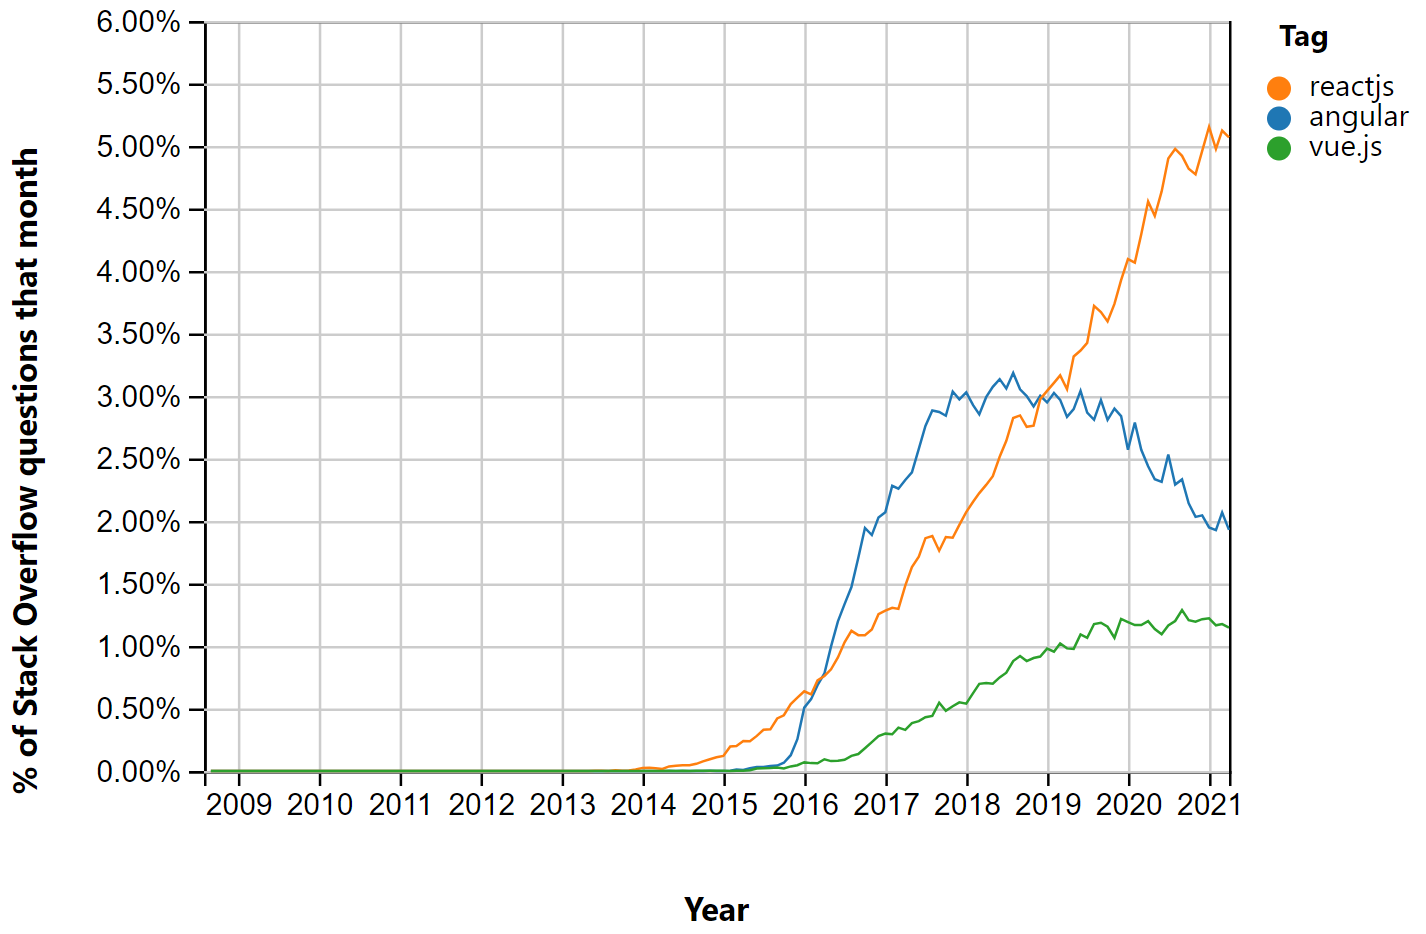
\includegraphics[width=\textwidth]{obrazky-figures/frameworkPopularityByQuestions.png}
\caption{Měsíční procentuální četnosti otázek na StackOverflow ohledně aplikačních rámců Angular, Vue, React. Převzato z \url{https://insights.stackoverflow.com/trends?tags=reactjs\%2Cvue.js\%2Cangular}}
\end{figure}
\FloatBarrier

Obrázek \ref{SOQuestions} znázorňuje měsíční procentuální četnosti otázek týkajících se daného aplikačního rámce na platformě Stack Overflow. Byla vybrána i knihovna React, protože trend úpadku Angularu nebyl tolik v prospěch Vue, jako spíše Reactu, u něhož lze pozorovat rostoucí trend.

\FloatBarrier
\begin{figure}[!htb]
\label{SOSurvey}
\centering
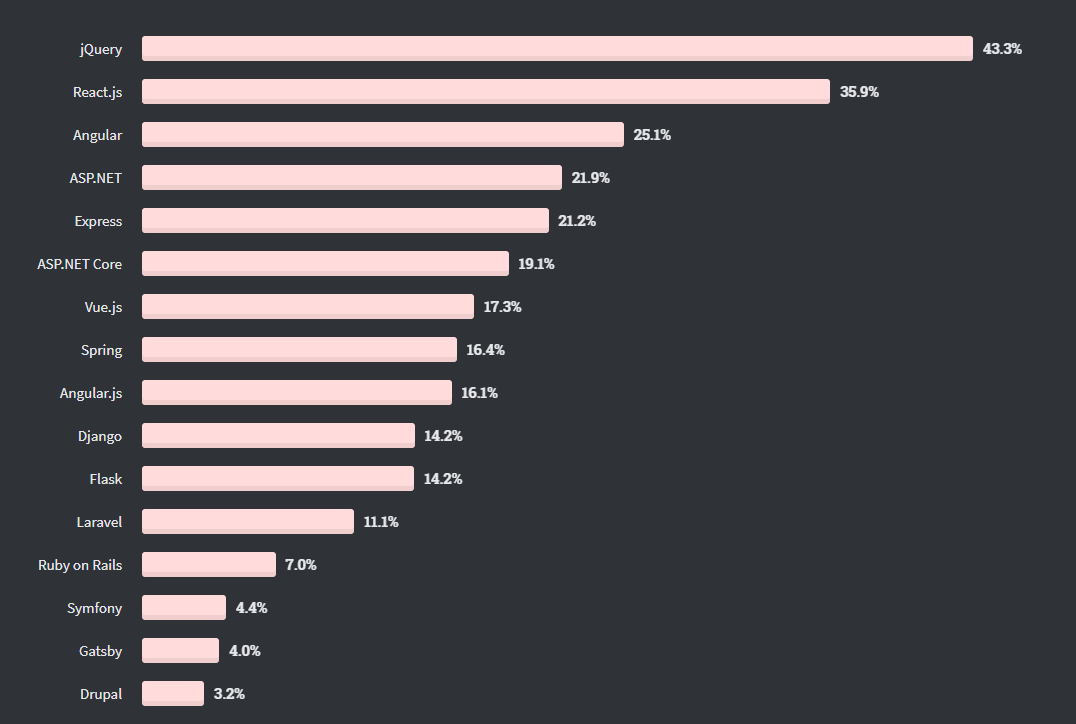
\includegraphics[width=\textwidth]{obrazky-figures/frameworkPopularityBySurvey.png}
\caption{Zastoupení využití javascriptových rámců a knihoven na základě dotazníku od společnosti StackOverflow. Převzato z \url{https://insights.stackoverflow.com/survey/2020#technology-web-frameworks}}
\end{figure}
\FloatBarrier

Stack Overflow také dělá průzkum mezi profesionálními vývojáři aplikací. Tato platforma zjišťuje, jaké technologie jsou nejvíce využívané. Na obrázku \ref{SOSurvey} je procentuální zastoupení použití daných rámců a knihoven u daných vývojářů, které vychází z dat z roku 2020. Zde Angular značně vede s 25,1 \% a Vue je na páté pozici se 17,3 \%.

\FloatBarrier
\begin{figure}[!htb]
\label{NpmDownloads}
\centering
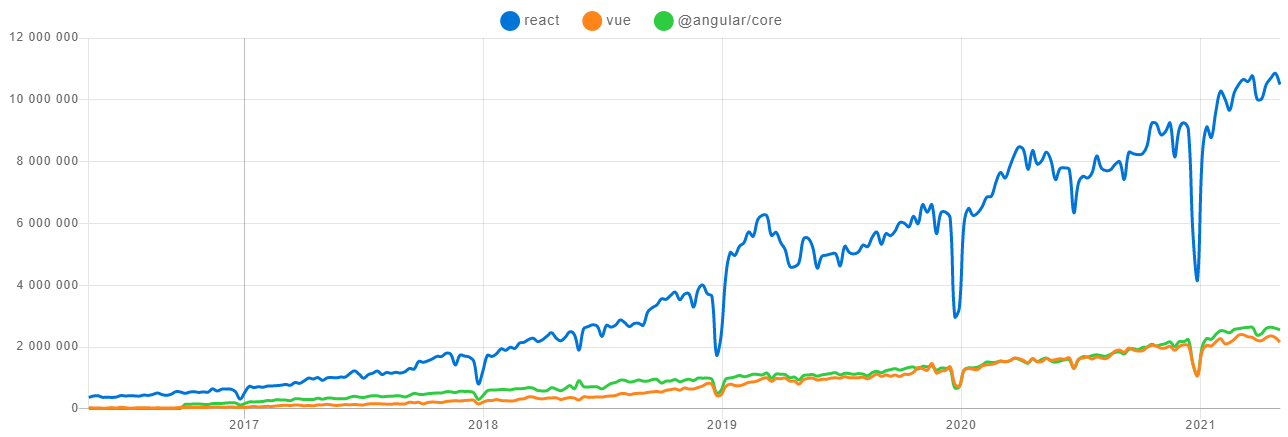
\includegraphics[width=\textwidth]{obrazky-figures/frameworkPopularityByDownloads.png}
\caption{Četnost stažení knihoven Angular, Vue a React z platformy npm. Převzato z \url{https://www.npmtrends.com/react-vs-vue-vs-@angular/core}}
\end{figure}
\FloatBarrier

V rámci platformy npm je možné sledovat počet stažení knihoven jednotlivých rámců. Kromě Angularu a Vue byl přidán také React pro lepší srovnání. Na obrázku \ref{NpmDownloads} lze pozorovat vývoj stahování těchto knihoven, přičemž je patrné, že React má nad Angularem i Vue výraznou převahu a tento trend má tendenci se časem prohlubovat. Vyšší četnost stažení knihoven Reactu může souviset s tím, že React je pouze knihovna, a tak má více použití. Angular i Vue dosahují srovnatelné četnosti stahování.

Závěrečným srovnáním je uživatelské hodnocení javascriptových aplikačních rámců na platformě GitHub. Jedná se sice pouze o subjektivní hodnocení, jež je ale přeci jen jistým ukazatelem popularity. Přední příčku zde zabírá rámec Vue, který zde obdržel více než 22 500 hvězd\cite{risingstars}. Na druhé příčce se nachází React, u kterého lze pozorovat 19 800 hvězd (tedy o 12 \% méně než Vue). Framework Angular pak zaujímá třetí pozici s 13 300 hvězdami, což je o 41 \% méně oproti Vue.


    \section{Shrnutí}
Na základě předchozího textu je patrné, že Angular je určený pro vývoj mohutnějších aplikací s komplexní vnitřní logikou. Angular svou striktností určuje chod vývoje aplikace, což podporuje týmový vývoj aplikací. Vue je oproti tomu jednoduše použitelný, lehký aplikačný rámec určený pro menší až střední projekty. Je velmi modulární a dá se dodatečně implement do jakékoliv aplikace, jak je patrné i z mnou vytvořené aplikace.
  \chapter{Závěr}
Cílem této práce bylo představit nástroje určené pro vývoj webových aplikací fungující na bázi JavaScriptu, navrhnout vhodnou demonstrační aplikaci za použití alespoň dvou nástrojů a tuto aplikaci realizovat. Dále bylo mým cílem srovnat vybrané nástroje na základě vybraných kritérií spolu se zkušenostmi z tvorby webové aplikace. Ná základě těchto kritérií považuji cíle práce za splněné.

Ve své práci popisuji teoretický základ týkající se základních nástrojů a praktik spojených s vývojem webové aplikace. Je zde také popsán jazyk JavaScript, technologie s ním spojené a samozřejmě také samotné javascriptové aplikační rámce pro vývoj, tedy Angular, Vue a React. Na základě rešerše byla navržena demonstrační aplikace pro použití dvou javascriptových aplikačních rámců, a to Angular a Vue. Tato aplikace byla úspěšně implementována jako webový portál pro prodej a správu vstupenek na koncerty a události. Aplikace využívá řady technologií, které aplikační rámce zpřístupňují. Angular zajišťuje komunikaci s databází v reálném čase, zpracovává většinu vnitřní logiky na straně klienta a dodává aplikaci pevnou logickou strukturu. Vue je použit jako rychlá a snadno modulovatelná webová komponenta zpracovávající data o vstupence do responzivní grafické šablony. Oba nástroje jsou dále na základě pozorovatelných aspektů porovnány.
Webová aplikační část pro prodej vstupenek je dostupná pod následujícím odkazem: \url{https://ticketeer-4d3d3.firebaseapp.com/}. Pro demonstraci případného použití se zde aplikace nachází v testovací šabloně. Aplikační část odpovídající za správu událostí a vstupenek je možné najít pod tímto odkazem: \url{https://ticketeer-4d3d3.firebaseapp.com/admin.html}. 

Práce by bylo možné rozšířit o srovnávací aspekty jako je například velikost souborů či rychlost zpracovávání, to by však vyžadovalo implementaci identické aplikace v obou aplikačních rámcích. Aplikace by dále mohla mít lépe nadesignované webové rozhraní, to však nebylo pro potřeby této práce nutné.

  
  % Kompilace po částech (viz výše, nutno odkomentovat)
  % Compilation piecewise (see above, it is necessary to uncomment it)
  %\subfile{projekt-01-uvod-introduction}
  % ...
  %\subfile{chapters/projekt-05-conclusion}


  % Pouzita literatura / Bibliography
  % ----------------------------------------------
\ifslovak
  \makeatletter
  \def\@openbib@code{\addcontentsline{toc}{chapter}{Literatúra}}
  \makeatother
  \bibliographystyle{bib-styles/Pysny/skplain}
\else
  \ifczech
    \makeatletter
    \def\@openbib@code{\addcontentsline{toc}{chapter}{Literatura}}
    \makeatother
    \bibliographystyle{bib-styles/Pysny/czplain}
  \else 
    \makeatletter
    \def\@openbib@code{\addcontentsline{toc}{chapter}{Bibliography}}
    \makeatother
    \bibliographystyle{bib-styles/Pysny/enplain}
  %  \bibliographystyle{alpha}
  \fi
\fi
  \begin{flushleft}
  \bibliography{projekt-20-literatura-bibliography}
  \end{flushleft}

  % vynechani stranky v oboustrannem rezimu
  % Skip the page in the two-sided mode
  \iftwoside
    \cleardoublepage
  \fi

  % Prilohy / Appendices
  % ---------------------------------------------
  \appendix
\ifczech
  \renewcommand{\appendixpagename}{Přílohy}
  \renewcommand{\appendixtocname}{Přílohy}
  \renewcommand{\appendixname}{Příloha}
\fi
\ifslovak
  \renewcommand{\appendixpagename}{Prílohy}
  \renewcommand{\appendixtocname}{Prílohy}
  \renewcommand{\appendixname}{Príloha}
\fi
%  \appendixpage

% vynechani stranky v oboustrannem rezimu
% Skip the page in the two-sided mode
%\iftwoside
%  \cleardoublepage
%\fi
  
\ifslovak
%  \section*{Zoznam príloh}
%  \addcontentsline{toc}{section}{Zoznam príloh}
\else
  \ifczech
%    \section*{Seznam příloh}
%    \addcontentsline{toc}{section}{Seznam příloh}
  \else
%    \section*{List of Appendices}
%    \addcontentsline{toc}{section}{List of Appendices}
  \fi
\fi
  \startcontents[chapters]
  \setlength{\parskip}{0pt} 
  % seznam příloh / list of appendices
  % \printcontents[chapters]{l}{0}{\setcounter{tocdepth}{2}}
  
  \ifODSAZ
    \setlength{\parskip}{0.5\bigskipamount}
  \else
    \setlength{\parskip}{0pt}
  \fi
  
  % vynechani stranky v oboustrannem rezimu
  \iftwoside
    \cleardoublepage
  \fi
  
  % Přílohy / Appendices
  \ifenglish
    \input{projekt-30-prilohy-appendices-en}
  \else
    \chapter{Obsah přiloženého paměťového média}

\begin{itemize}
    \item doc - Složka obsahující text technické zprávy a jeho zdrojový kód.
    \item src - Složka obsahující zdrojový kód k aplikaci:
        \begin{itemize}
            \item ticketeer - Složka obsahující Angular část aplikace
            \item tickets-component-wc - Složka obsahující Vue část aplikace
        \end{itemize}
    \item README.txt - Textový soubor obsahující návod pro apliakci.
\end{itemize}                   
  \fi
  
  % Kompilace po částech (viz výše, nutno odkomentovat)
  % Compilation piecewise (see above, it is necessary to uncomment it)
  %\subfile{projekt-30-prilohy-appendices}
  
\end{document}
